\documentclass[a4paper,11pt]{article}

\usepackage[T1]{fontenc}
\usepackage[utf8]{inputenc}
\usepackage{lmodern}
\usepackage[english]{babel}
\usepackage{microtype}
\usepackage{iftex}
\usepackage[a4paper, top=2.8cm, bottom=2.3cm, left=2.8cm, right=2.3cm, headheight=32pt, headsep=14pt]{geometry}
\usepackage{setspace}
\setstretch{1.03}
\setlength{\parindent}{1.2em}
\setlength{\parskip}{3pt}

\usepackage{bxcalc}
\usepackage{float}
\usepackage[svgnames]{xcolor}
\usepackage{tikz}
\usetikzlibrary{shapes.geometric,shapes.misc,positioning,fit,arrows.meta,calc}
\usepackage{graphicx}
\usepackage{amsmath, amssymb}
\usepackage{enumitem}
\setlist{noitemsep}
\usepackage{caption}
\captionsetup{font=small, labelfont=bf}
\usepackage{tabularray}
\usepackage{pdflscape}
\usepackage{xurl}
\usepackage{listings}
\usepackage{titlesec}
\usepackage{titletoc}
\usepackage{tocloft}
\usepackage{fancyhdr}
\usepackage{lastpage}
\usepackage{chngcntr}

% ---------- numbering as in the HCMUT template: 1 Section / 5.1 Subsection ----------
\counterwithin{figure}{section}
\counterwithin{table}{section}
\AtBeginDocument{\counterwithin{lstlisting}{section}}
\titleformat{\section}{\Large\bfseries}{\thesection}{1em}{}
\titleformat{\subsection}{\large\bfseries}{\thesubsection}{1em}{}
\titleformat{\subsubsection}{\normalsize\bfseries}{\thesubsubsection}{1em}{}
\titlespacing*{\section}{0pt}{20pt}{10pt}
\titlespacing*{\subsection}{0pt}{14pt}{6pt}
\titlespacing*{\subsubsection}{0pt}{10pt}{4pt}
\setcounter{secnumdepth}{3}
\setcounter{tocdepth}{2}

% ---------- table of contents style (bold sections, dotted subsections) ----------
\renewcommand{\cftsecfont}{\bfseries}
\renewcommand{\cftsecpagefont}{\bfseries}
\renewcommand{\cftsecleader}{\hfill}
\renewcommand{\cftsecaftersnum}{}
\setlength{\cftbeforesecskip}{6pt}
\setlength{\cftbeforesubsecskip}{1pt}
\renewcommand{\cftdot}{.}
\renewcommand{\cftdotsep}{2}
\renewcommand{\cftsecleader}{\bfseries\cftdotfill{\cftsecdotsep}}
\renewcommand{\cftsecdotsep}{\cftdotsep}
\renewcommand{\cftfigfont}{\small}
\renewcommand{\cfttabfont}{\small}
\setlength{\cftfigindent}{1em}
\setlength{\cfttabindent}{1em}
\renewcommand{\cftfigpresnum}{}
\renewcommand{\cfttabpresnum}{}
\setlength{\cftfignumwidth}{2.6em}
\setlength{\cfttabnumwidth}{2.6em}
\renewcommand{\cftloftitlefont}{\Large\bfseries}
\renewcommand{\cftlottitlefont}{\Large\bfseries}
\renewcommand{\contentsname}{Contents}
\renewcommand{\cfttoctitlefont}{\Large\bfseries}
\renewcommand{\cftaftertoctitle}{\par\vspace{-4pt}}

% ---------- header / footer ----------
\newcommand{\hdrtext}{\ttfamily\footnotesize Ho Chi Minh City University of Technology\\Faculty of Computer Science and Engineering}
\fancypagestyle{body}{\fancyhf{}
  \fancyhead[R]{\hdrtext}
  \fancyfoot[C]{\small\thepage}
  \renewcommand{\headrulewidth}{0.4pt}\renewcommand{\footrulewidth}{0pt}}
\fancypagestyle{front}{\fancyhf{}
  \fancyhead[L]{
\includegraphics[height=0.9cm]{images/logo.png}}
  \fancyhead[R]{\hdrtext}
  \fancyfoot[C]{\small\thepage}
  \renewcommand{\headrulewidth}{0.4pt}\renewcommand{\footrulewidth}{0pt}}
\fancypagestyle{plain}{\fancyhf{}\fancyfoot[C]{\small\thepage}\renewcommand{\headrulewidth}{0pt}}
\fancypagestyle{blank}{\fancyhf{}\renewcommand{\headrulewidth}{0pt}}

\usepackage[unicode, colorlinks=true, linkcolor=DodgerBlue, urlcolor=DodgerBlue, citecolor=DodgerBlue, breaklinks=true,
  pdftitle={Design of an E-Learning System with AI Integration},
  pdfauthor={Nguyen Ngoc Sang, Nguyen Huu Hao, Pham Quang Tuan}]{hyperref}

% ---------- listings ----------
\lstset{
    basicstyle=\ttfamily\small,
    keywordstyle=\bfseries\color{NavyBlue},
    commentstyle=\itshape\color{Gray},
    stringstyle=\color{DarkGreen},
    numbers=left, numberstyle=\tiny\color{Gray}, numbersep=6pt,
    frame=tb, rulecolor=\color{Gray}, backgroundcolor=\color{gray!6},
    breaklines=true, columns=fullflexible, keepspaces=true, showstringspaces=false,
    captionpos=t, xleftmargin=12pt, xrightmargin=4pt,
}
\lstdefinelanguage{SQLpg}{
    morekeywords={CREATE,TABLE,FUNCTION,TRIGGER,INDEX,UNIQUE,PRIMARY,KEY,REFERENCES,ON,DELETE,CASCADE,RESTRICT,NOT,NULL,DEFAULT,CHECK,BEFORE,INSERT,UPDATE,FOR,EACH,ROW,EXECUTE,RETURNS,AS,DECLARE,BEGIN,END,IF,THEN,RETURN,SELECT,FROM,WHERE,AND,OR,INTO,RAISE,EXCEPTION,USING,ERRCODE,LANGUAGE,REPLACE,OF,WITH,IN,TIME,TIMESTAMPTZ,UUID,VARCHAR,INTEGER,BOOLEAN,DATE,SMALLINT,JSONB,TEXT,NUMERIC},
    sensitive=false, morecomment=[l]{--}, morestring=[b]'
}
\lstdefinelanguage{TS}{
    morekeywords={import,from,const,let,async,await,function,return,if,else,throw,new,export,type,interface,try,catch},
    sensitive=true, morecomment=[l]{//}, morestring=[b]', morestring=[b]"
}
\ExplSyntaxOn
\NewDocumentCommand{\code}{m}{%
  \tl_set:Nx \l_tmpa_tl { \detokenize{#1} }
  \tl_replace_all:Nxx \l_tmpa_tl { \char_generate:nn{95}{12} } { \char_generate:nn{95}{12} \exp_not:N\allowbreak }
  \tl_replace_all:Nxx \l_tmpa_tl { \char_generate:nn{47}{12} } { \char_generate:nn{47}{12} \exp_not:N\allowbreak }
  \texttt{\l_tmpa_tl}}
\ExplSyntaxOff

\begin{document}

% ================= Cover page =================
\thispagestyle{blank}
\begin{titlepage}
\centering
{\small VIETNAM NATIONAL UNIVERSITY HO CHI MINH CITY\\
HO CHI MINH CITY UNIVERSITY OF TECHNOLOGY\\
FACULTY OF COMPUTER SCIENCE AND ENGINEERING\par}
\vspace{1.4cm}

\includegraphics[height=3.6cm]{images/logo.png}\par
\vspace{1.0cm}
{\Large\textbf{Specialized Project (CO4029)}\par}
\vspace{0.6cm}
\rule{0.88\textwidth}{0.8pt}\par
\vspace{0.9cm}
{\large Report --- Semester 1, 2026--2027 \\ Project code: HK261-DAGD1-480\par}
\vspace{0.5cm}
{\Huge\bfseries Design of an E-Learning System with AI Integration\par}
\vspace{0.7cm}
\rule{0.88\textwidth}{0.8pt}\par
\vspace{1.2cm}
\begin{tabular}{@{}r@{\hspace{0.6em}}l@{\hspace{1.2em}}l@{}}
Advisor: & Dr. Nguyen Quoc Minh & \\[4pt]
Students: & Nguyen Ngoc Sang & 2353046\\
 & Nguyen Huu Hao & 2352296\\
 & Pham Quang Tuan & 2353275\\
\end{tabular}
\vfill
HO CHI MINH CITY, NOVEMBER 2026
\end{titlepage}
\newpage

% ================= Abstract and acknowledgements =================
\pagestyle{front}
\pagenumbering{roman}
\setcounter{page}{1}
\section*{Abstract}
\addcontentsline{toc}{section}{Abstract}

Learning Management Systems (LMS) are now the backbone of blended and online teaching at universities. At Ho Chi Minh City University of Technology (HCMUT), students and lecturers use the BKeL portal, which is built on Moodle, to access course material, submit work and follow their timetable. Despite its maturity, a generic LMS does not model several routine academic processes in a way that is convenient for a single course: a course offered as a numbered sequence of fifteen sessions, in-class attendance that cannot be faked remotely, and per-session statistics that a lecturer can read at a glance.

This report presents the first part of the specialized project (CO4029) \emph{``Design of an E-Learning System with AI Integration''} (project code HK261-DAGD1-480): the design and implementation of the e-learning platform itself. The platform reproduces the look and feel of the BKeL portal and adds the academic workflow of a real class: semesters, course offerings, enrollment with a capacity limit, a fifteen-session schedule with a weekly timetable, learning materials per session, and an in-class attendance mechanism based on a short-lived, randomly generated four-digit PIN that is opened by the lecturer and entered by students.

The report documents the requirements (seven use cases in Cockburn's format), the architecture (a Next.js~14 front end, an Express/TypeScript REST API, and a PostgreSQL database), and the relational schema of fourteen tables in third normal form, including the constraints and the trigger that protect data integrity. It also describes the dataset prepared for the pilot course \emph{Data Structures and Algorithms} (CO2003): a fifteen-session outline and a bank of forty multiple-choice questions labeled with eleven skills. The current prototype, its security measures and its known limitations are described honestly, and the last chapter gives a week-by-week plan for the second semester (HK262) in which the system will be completed, evaluated with users and extended with the intelligent learning-support features of the full project.

\bigskip
\noindent\textbf{Keywords:} learning management system, e-learning, BKeL, Moodle, PostgreSQL, REST API, attendance, Next.js.

\section*{Acknowledgements}
\addcontentsline{toc}{section}{Acknowledgements}

The team would like to thank Dr.\ Nguyen Quoc Minh, our supervisor, for his guidance during the biweekly meetings. His feedback after the third meeting, which asked us to turn the first prototype into a complete university-grade system before anything else, shaped the direction of this report. We also thank the Faculty of Computer Science and Engineering, HCMUT, for the learning environment, and our classmates who tested the prototype and gave us honest comments.



% ================= Contents and lists =================
\clearpage
\hypersetup{linkcolor=black}
\tableofcontents
\listoffigures
\hypersetup{linkcolor=DodgerBlue}
\clearpage
\section*{List of Abbreviations}
\addcontentsline{toc}{section}{List of Abbreviations}

\small\begin{tblr}{colspec={Q[l,1.6cm]X[l]}, rowsep=0pt}
API & Application Programming Interface\\
BKeL & HCMUT e-Learning portal (Moodle-based)\\
CAS & Central Authentication Service\\
CRUD & Create, Read, Update, Delete\\
CSS & Cascading Style Sheets\\
ERD & Entity-Relationship Diagram\\
HCMUT & Ho Chi Minh City University of Technology\\
HTTP & Hypertext Transfer Protocol\\
JSON & JavaScript Object Notation\\
JWT & JSON Web Token\\
LMS & Learning Management System\\
PIN & Personal Identification Number\\
RBAC & Role-Based Access Control\\
REST & Representational State Transfer\\
SPA & Single-Page Application\\
SQL & Structured Query Language\\
UC & Use Case\\
UI/UX & User Interface / User Experience\\
UUID & Universally Unique Identifier\\
\end{tblr}

\clearpage


\pagestyle{body}
\pagenumbering{arabic}
\setcounter{page}{1}

\section{Introduction}
\label{ch:intro}

\subsection{Context and Motivation}

Over the last two decades, the Learning Management System has become the standard infrastructure through which universities deliver courses, collect assignments and communicate with students~\cite{ellis2009field}. A systematic review of LMS adoption in higher education shows that institutions mostly choose between a small number of mature platforms, and that Moodle is one of the most widely used open-source options~\cite{kasim2016choosing, dougiamas2003moodle}. Ho Chi Minh City University of Technology (HCMUT) follows this pattern: its BKeL portal is a customized Moodle deployment that students open every day to see their courses.

A general-purpose LMS has to serve every faculty and every teaching style, so its data model is deliberately generic: a course contains topics, a topic contains activities. This generality is a strength for the platform operator, but it leaves some everyday needs of a lecturer to plugins and manual conventions. In a typical engineering course at HCMUT, the lecturer meets the same group of students for fifteen weekly sessions in a fixed room. The lecturer needs to know who attended each session, how the attendance of the whole class evolves over the semester, and which students are at risk of failing the attendance requirement. Attendance matters in practice: a meta-analysis of the literature found that class attendance is a strong predictor of university grades, stronger than several other commonly studied predictors~\cite{crede2010class}, and large-scale studies of student behavior confirm the link between regular attendance and academic performance~\cite{kassarnig2018academic}.

At the same time, in-class attendance is easy to abuse. A plain ``tick'' button or a QR code posted on a slide can be shared with absent classmates through a messaging application within seconds. A mechanism is needed that proves the student is present while the lecturer is running the session, and that is simple enough to be used in the first five minutes of a lecture.

\subsection{Problem Statement}

The project aims at an e-learning platform that behaves like a real university LMS rather than a collection of quiz pages. Concretely, the problems addressed in this report are:

\begin{enumerate}
    \item \textbf{Academic structure.} The system must represent semesters, courses, course classes (an offering of a course in one semester, e.g.\ CO2003--CC01 in HK261), enrollments with a maximum capacity, and the fifteen numbered sessions of each class with date, time and room.
    \item \textbf{Trustworthy attendance.} The system must let the lecturer open an attendance window in class and generate a random PIN that is valid for a short time. Students check in with the PIN. The system must prevent duplicate check-ins, guessing of the PIN and check-in after the window is closed.
    \item \textbf{Course content per session.} Every session must have its own materials (slides, code, videos) so that students can find what belongs to ``Week 7'' without searching.
    \item \textbf{Reports for the lecturer.} The lecturer must see enrollment against capacity, the participation rate of every session and the attendance rate of every student.
    \item \textbf{Familiar user experience.} The interface must feel familiar to HCMUT users: the BKeL color scheme, the Moodle-style course cards and activity icons, and a clear separation between the lecturer and the student role from the login screen.
    \item \textbf{A sound data foundation.} The relational schema must be normalized, protect its invariants through constraints and a trigger, and keep the data produced by quizzes in a form that later analysis can use.
\end{enumerate}

\subsection{Objectives and Scope}

The general objective of the project is to build an adaptive e-learning system for university teaching. Following the feedback of the supervisor after the third meeting (25 October 2026), the work is organized in two phases. This report covers \textbf{Phase~1}: a complete, well-engineered e-learning system. Phase~2, planned for the second semester (HK262), extends the system with intelligent learning support and evaluates it with real users; it is only outlined in Section~\ref{ch:plan}.

The specific objectives of Phase~1 are to:

\begin{itemize}
    \item analyze the requirements of lecturers and students and express them as use cases;
    \item design a three-tier architecture and a relational schema in third normal form (3NF);
    \item implement a REST API with authentication, authorization and the attendance mechanism;
    \item implement a front-end prototype that follows the BKeL visual identity;
    \item prepare a realistic dataset for one pilot course, \emph{Data Structures and Algorithms} (CO2003), including a fifteen-session outline and a labeled bank of forty multiple-choice questions;
    \item document the design, the known limitations and a plan for the next semester.
\end{itemize}

\paragraph{Scope.} The pilot course is CO2003 (4 credits), class CC01, in the active semester HK261. The report covers: authentication and roles, schedule and timetable, session materials, PIN-based attendance, enrollment and attendance statistics, and the question bank. It does \emph{not} cover payment, grading workflows, a forum, or integration with the real HCMUT CAS server; the CAS login page in the prototype is a visual reproduction.

\subsection{Contributions}

The main contributions of the first phase are:

\begin{enumerate}
    \item a \textbf{use-case model} of seven use cases, of which UC5--UC7 (sessions and timetable, PIN attendance, attendance statistics) are specified in full detail;
    \item a \textbf{fourteen-table relational schema} with composite foreign keys, check constraints, partial unique indexes and a row-locking trigger that guarantees class capacity under concurrent enrollment;
    \item a \textbf{PIN attendance protocol} that combines a cryptographically secure random generator, a short expiry, a background sweep, a constant-time comparison, one record per student and session, and rate limiting;
    \item a \textbf{front-end prototype} with 100\% vector icons, light and dark themes, and the pages ``My courses'', ``Sessions'', ``Attendance'', ``Timetable'', ``Statistics'' and ``Quiz'';
    \item a \textbf{pilot dataset} for CO2003: fifteen sessions, eleven skill labels and forty questions with answers and explanations.
\end{enumerate}

\subsection{Team and Division of Work}

The project is carried out by three students under the supervision of Dr.\ Nguyen Quoc Minh. Table~\ref{tab:team} shows the responsibilities of each member.

\begin{table}[H]
\centering
\caption{Team members and responsibilities}
\label{tab:team}
\begin{tblr}{colspec={Q[l,3.4cm]Q[l,2.2cm]X[l]}, row{1}={font=\bfseries}, hline{1,Z}={0.8pt}, hline{2}={0.4pt}, rowsep=3pt}
Member & Student ID & Responsibility\\
Nguyen Ngoc Sang & 2353046 & Overall architecture, Next.js front end (BKeL portal), integration, coordination\\
Nguyen Huu Hao & 2352296 & PostgreSQL schema (3NF), Express/TypeScript REST API, attendance PIN security, triggers\\
Pham Quang Tuan & 2353275 & Requirements analysis and use cases, CO2003 dataset, session outline, question bank labeled by skill\\
\end{tblr}
\end{table}

\subsection{Report Organization}

The remainder of this report is organized as follows. Section~\ref{ch:background} reviews the background: LMS platforms, the BKeL portal and the technologies used. Section~\ref{ch:req} presents the requirements and use cases. Section~\ref{ch:design} describes the methodology, the overall pipeline, the architecture and the database design. Section~\ref{ch:impl} describes the implementation, the prototype and the dataset. Section~\ref{ch:eval} reports the testing performed so far and discusses limitations. Section~\ref{ch:plan} concludes and gives the plan for weeks 1--15 of the graduation project in HK262.

\subsection{Milestones of the Specialized Project}

Table~\ref{tab:meetings} lists the meetings with the supervisor and the state of each milestone at the time of writing.

\begin{table}[H]
\centering
\caption{Meetings with the supervisor and project milestones}
\label{tab:meetings}
\begin{tblr}{colspec={Q[l,1.2cm]Q[l,2.6cm]X[l]Q[l,2.4cm]}, row{1}={font=\bfseries}, hline{1,Z}={0.8pt}, hline{2}={0.4pt}, rowsep=3pt}
No. & Date & Content & Status\\
1 & 27/09/2026 & Agree on the outline and division of responsibilities & Done\\
2 & 11/10/2026 & Survey of background material and the plan of the system & Done\\
3 & 25/10/2026 & Initial architecture, four core use cases; feedback: strengthen the database and add university-level LMS features & Done\\
4 & 10/11/2026 & Database ERD (14 tables), pilot course CO2003 (15 sessions, timetable, PIN attendance, statistics) on the BKeL-style portal & Done\\
5 & 22/11/2026 & Review of the report draft and of the completed system (report milestones: at least 30 pages on 15/11) & Planned\\
6--7 & 12/2026 & Testing, refinement and report revision (at least 50 pages on 30/11 and 70 pages on 15/12) & Planned\\
8 & 31/12/2026 & Final defense of the specialized project (CO4029) & Planned\\
\end{tblr}
\end{table}

\section{Background and Related Work}
\label{ch:background}

This section reviews the concepts and technologies on which the system is built. It starts from the role of an LMS and the BKeL portal, continues with the design principles and software-engineering practices adopted, and ends with a description of the technology stack and the reasons for choosing it.

\subsection{Learning Management Systems}

\subsubsection{Definition and Typical Functions}

A Learning Management System is a software application for the administration, documentation, tracking, reporting and delivery of educational courses~\cite{ellis2009field}. Common functions are: user and role management, course catalog, delivery of learning material, assessment (quizzes and assignments), communication tools, and reporting. The success of an e-learning system depends on several dimensions, including system quality, information quality, service quality and the satisfaction of learners and instructors~\cite{alfraihat2020evaluating}. For this project these dimensions translate into three practical concerns: the interface must be easy to use, the data shown must be correct and up to date, and the system must be reliable during a lecture.

\subsubsection{Moodle and BKeL}

Moodle is an open-source course management system based on a social-constructivist pedagogy~\cite{dougiamas2003moodle}. Its documentation describes the structure that students of HCMUT know well: a \emph{course} contains \emph{sections}, and a section contains \emph{activities and resources} such as files, pages, quizzes and forums~\cite{moodledocs}. The BKeL portal of HCMUT is built on Moodle and is combined with the university's Central Authentication Service (CAS). A user logs in through the CAS page, lands on a dashboard that lists enrolled courses as cards, and enters a course page organized in weekly or topic sections.

The visual language of BKeL has become part of the daily habits of students: a teal-blue header, a course card with a geometric pattern, small icons for each activity type, and a left-hand navigation drawer. A new system that wants to be adopted should not ask users to learn a new interface for the same tasks. For this reason, the prototype of this project deliberately keeps the BKeL visual identity (primary color \texttt{\#008299}, Moodle-style cards and activity icons) while improving details such as spacing, motion and a dark theme.

\subsubsection{Limitations of a Generic LMS for Class-Level Operations}

Moodle is highly extensible, but several class-level operations are not part of its core data model. Table~\ref{tab:gap} summarizes the gaps that motivated this project. We want to be precise: these are gaps in \emph{the default data model and workflow}, not in what an administrator can achieve with plugins.

\begin{table}[H]
\centering
\caption{Class-level needs and how they map onto a generic LMS and onto the proposed system}
\label{tab:gap}
\begin{tblr}{colspec={Q[l,3.3cm]X[l]X[l]}, row{1}={font=\bfseries}, hline{1,Z}={0.8pt}, hline{2}={0.4pt}, rowsep=3pt}
Need & Generic LMS (default) & Proposed system\\
Offering of a course in a semester with a capacity & Course and enrollment methods; capacity usually handled by the registration system & First-class entities \code{semesters}, \code{course_classes}, \code{enrollments}; capacity enforced by a database trigger\\
Exactly 15 numbered sessions with date, time and room & Weekly sections with free-form dates & \code{course_sessions} with \code{session_number} in $[1,15]$ and a transactional bulk creation\\
Proof of presence in class & Attendance via plugin or manual tick & Random four-digit PIN with expiry, rate limit and one record per student and session\\
Participation per session and per student & Reports depend on the plugin & Dedicated endpoint and statistics page\\
Skill label per question & Question categories (free-form) & \code{skills} table; a question references exactly one skill by foreign key\\
\end{tblr}
\end{table}

\subsection{Attendance Management}

Attendance can be recorded in several ways: a paper roll call, a tick on a list, a QR code shown on a screen, biometric systems, or a code that is announced in class. Each has a different trade-off between effort, cost and resistance to proxy attendance (a classmate checking in for an absent student).

\begin{itemize}
    \item \textbf{Roll call} is reliable but consumes lecture time proportional to the number of students.
    \item \textbf{Static QR codes} are fast but can be photographed and sent to absent students.
    \item \textbf{Biometric or location-based systems} are strong but require special hardware or permissions and raise privacy concerns.
    \item \textbf{A short-lived PIN} shown on the lecturer's screen requires physical presence in the room (or at least a live view of the screen), costs a few seconds, and needs no additional hardware.
\end{itemize}

We chose the PIN approach. A four-digit PIN has only 10\,000 possible values, so on its own it is weak against a brute-force attack from a logged-in student. The system therefore combines it with three controls: a short validity period of ten to fifteen minutes, a limit of five failed attempts per student and session in a fifteen-minute window (HTTP status 429, defined in~\cite{rfc6585}), and the requirement that the student is enrolled in the class. The effect of these controls is analyzed in Section~\ref{sec:pin-security}. The importance given to attendance is justified by the evidence that attendance is associated with grades~\cite{crede2010class, kassarnig2018academic}.

\subsection{Software Architecture Principles}

\subsubsection{Layered and Client--Server Architecture}

The system adopts a three-tier layered architecture: presentation, application and persistence. Layering separates concerns and allows each tier to evolve independently~\cite{bass2021software, fowler2002patterns}. The client--server style also makes it possible to scale the stateless API horizontally~\cite{fielding2000architectural}.

\subsubsection{REST}

The API follows the REST architectural style: resources are identified by URLs, the standard HTTP methods express the intent of a request, and each request carries all the information needed to process it~\cite{fielding2000architectural}. Message bodies use JSON~\cite{rfc8259}. The semantics of methods and status codes follow the HTTP specification~\cite{rfc9110}. Stateless requests simplify the deployment because any instance of the API can serve any request.

\subsubsection{Authentication and Authorization}

Authentication uses JSON Web Tokens~\cite{rfc7519}. After a successful login the server signs a token with a secret key and the client sends it in the \texttt{Authorization} header of later requests. Authorization is role based: a user is a student, an instructor or an administrator, and every route declares which roles may call it. Passwords are never stored in clear text; they are hashed with bcrypt, a password hashing scheme that includes a salt and an adaptive cost so that it can be made slower as hardware improves~\cite{provos1999bcrypt}. The recommendations of NIST for digital identity~\cite{nist80063b} and the OWASP application security verification standard~\cite{owaspasvs} guide the minimum requirements for password storage and for rate limiting of authentication-like operations.

\subsection{Relational Data Modeling}

\subsubsection{Relational Model and Normalization}

The relational model~\cite{codd1970relational} represents data as relations (tables) and offers a declarative query language. The entity-relationship model~\cite{chen1976entity} is the usual notation for conceptual design. A schema is in third normal form (3NF) when every non-key attribute depends on the key, the whole key and nothing but the key; textbooks such as~\cite{silberschatz2019database} and~\cite{elmasri2015fundamentals} describe the normal forms and the decomposition process. We use 3NF as a design rule for the fourteen tables of the system, and we accept a small number of deliberate exceptions that are documented in Section~\ref{sec:normalization}.

\subsubsection{Integrity Constraints and Triggers}

Declarative constraints (primary keys, foreign keys, \texttt{UNIQUE} and \texttt{CHECK}) let the database engine itself reject invalid data, so that integrity does not depend on every application path being correct. Triggers are used where a rule involves several rows, such as ``the number of enrolled students must not exceed the capacity of the class''. Because such a rule reads data and then writes data, two concurrent transactions can both read ``59 of 60'' and both insert. This is a classical concurrency anomaly; the SQL isolation levels and their anomalies are analyzed in~\cite{berenson1995critique}, and the more general theory of concurrency control in~\cite{bernstein1981concurrency}. The system prevents the anomaly with an explicit row lock (\texttt{SELECT ... FOR UPDATE}) taken on the class row inside the trigger~\cite{postgresdocs}.

\subsection{Technologies Used}

\subsubsection{Front End: Next.js and React}

The front end is written with Next.js~14 using the App Router, on top of React~18~\cite{nextjsdocs, reactdocs}. The pages are components; global styling uses CSS custom properties (design tokens) so that the light and dark themes are switched by changing the values of the variables. All icons are inline SVG so that they remain sharp at every size and need no external font.

\subsubsection{Back End: Node.js, Express and TypeScript}

The API runs on Node.js with the Express framework~\cite{nodedocs, expressdocs} and is written in TypeScript~\cite{typescriptdocs}. Static typing catches a whole class of errors (for example, a missing field of a database row) at compile time rather than during a lecture. The \texttt{pg} driver is used with parameterized queries to avoid SQL injection, which is listed among the most common web application risks by OWASP~\cite{owasptop10}.

\subsubsection{Database: PostgreSQL}

PostgreSQL~15 is used as the database. It supports \texttt{UUID} generation through the \texttt{pgcrypto} extension, partial unique indexes, composite foreign keys, \texttt{JSONB} columns, PL/pgSQL triggers and explicit row locks~\cite{postgresdocs}. These features are used in the schema described in Section~\ref{ch:design}.

\subsubsection{Tools and Practices}

Source code is managed with Git~\cite{chacon2014progit}. The system is developed incrementally with short iterations and frequent feedback from the supervisor, in the spirit of agile development~\cite{beck2001agile, sommerville2016software}. Containerization with Docker~\cite{merkel2014docker} and a continuous-delivery pipeline~\cite{humble2010continuous} are planned for the next semester (Section~\ref{ch:plan}).

\subsection{Usability and Accessibility}

Usability is treated as a quality attribute with measurable criteria. Nielsen's usability heuristics~\cite{nielsen1993usability} guided the design of the interface: visibility of system status (the attendance countdown), consistency with the BKeL conventions, error prevention (disabling the check-in button until four digits are typed), and recognition rather than recall (icons and labels together). For accessibility the Web Content Accessibility Guidelines~\cite{wcag21} are used as a reference, in particular the contrast ratio of text and the availability of keyboard navigation. The System Usability Scale~\cite{brooke1996sus, bangor2008empirical} is planned as the instrument for the user study in HK262.

\section{Requirements Analysis}
\label{ch:req}

This section states what the system must do. Requirements were collected from three sources: the observation of how the BKeL portal is used by students and lecturers of HCMUT, the guidance of the supervisor at the biweekly meetings, and the structure of the pilot course CO2003. Functional requirements are expressed as use cases in the format proposed by Cockburn~\cite{cockburn2001writing}, which derives from the use-case-driven approach of Jacobson et al.~\cite{jacobson1992object}. Diagrams follow UML notation~\cite{fowler2004uml}.

\subsection{Stakeholders and Actors}

Table~\ref{tab:actors} lists the actors of the system.

\begin{table}[H]
\centering
\caption{Actors of the system}
\label{tab:actors}
\begin{tblr}{colspec={Q[l,3cm]X[l]}, row{1}={font=\bfseries}, hline{1,Z}={0.8pt}, hline{2}={0.4pt}, rowsep=1.5pt, rows={font=\small}}
Actor & Description\\
Student & Logs in, sees the enrolled courses, the timetable and the materials of each session, checks in with the PIN, and takes practice quizzes.\\
Lecturer (Instructor) & Manages the sessions of a class, opens and closes attendance, reviews attendance and enrollment statistics, and maintains the question bank.\\
Administrator & Provisions lecturer and administrator accounts, manages semesters and course catalog.\\
System (timer) & Closes an attendance window automatically when its expiry time has passed.\\
\end{tblr}
\end{table}

\subsection{Functional Requirements}

The functional requirements are grouped by module. The identifiers are used in the traceability tables of Section~\ref{ch:impl}.

\begin{table}[H]
\centering
\caption{Functional requirements}
\label{tab:fr}
\begin{tblr}{colspec={Q[l,1.3cm]X[l]Q[l,2.2cm]}, row{1}={font=\bfseries}, hline{1,Z}={0.8pt}, hline{2}={0.4pt}, rowsep=1.5pt, rows={font=\small}}
ID & Requirement & Use case\\
FR1 & A user can register (as a student) and log in with e-mail and password; lecturers and administrators are provisioned by an administrator. & UC1\\
FR2 & The system shows the user's courses for the active semester as cards. & UC1\\
FR3 & A student can enroll in a class; the number of enrolled students must never exceed the maximum capacity of the class. & UC5, UC7\\
FR4 & A lecturer can create the fifteen sessions of a class in one operation, or one session at a time, and can edit or delete a session. & UC5\\
FR5 & The system validates sessions: unique number in $[1,15]$, end time after start time, and no conflict. & UC5\\
FR6 & A student sees a weekly timetable with the sessions of the classes in which he or she is enrolled; the current session is highlighted. & UC5\\
FR7 & Each session has an ordered list of materials of type slide, code or video. & UC1, UC5\\
FR8 & A lecturer can open an attendance window; the system generates a random four-digit PIN and an expiry time of 10--15 minutes. & UC6\\
FR9 & A student can check in with the PIN; the system records one record per student and session. & UC6\\
FR10 & The system rejects check-in when the window is closed or expired, when the student is not enrolled, or after five failed attempts in fifteen minutes. & UC6\\
FR11 & A lecturer can close attendance early and can mark attendance manually (present, absent, late, excused). & UC6\\
FR12 & A lecturer can see enrollment against capacity, the participation rate per session, and the attendance rate per student. & UC7\\
FR13 & A student can take a multiple-choice quiz of a session; each answer is stored as a separate interaction record. & UC2\\
FR14 & A lecturer can create questions with four options and assign a skill label. & UC3\\
FR15 & The user can switch between light and dark themes; the choice is remembered. & ---\\
\end{tblr}
\end{table}

\subsection{Non-Functional Requirements}

\begin{table}[H]
\centering
\caption{Non-functional requirements}
\label{tab:nfr}
\begin{tblr}{colspec={Q[l,1.3cm]Q[l,2.7cm]X[l]}, row{1}={font=\bfseries}, hline{1,Z}={0.8pt}, hline{2}={0.4pt}, rowsep=1.5pt, rows={font=\small}}
ID & Quality & Requirement\\
NFR1 & Security & Passwords are stored only as bcrypt hashes; API calls other than login and registration require a valid JWT; the answer key of a question is never sent to students; PIN check-in is rate limited.\\
NFR2 & Integrity & Invariants (capacity, uniqueness of attendance, valid time ranges, valid PIN format) are enforced by the database and not only by the application.\\
NFR3 & Concurrency & Concurrent enrollment of many students into the same class must not exceed the capacity.\\
NFR4 & Usability & The interface follows the BKeL visual identity; all primary actions are reachable in at most three clicks; no emoji or raster icons are used.\\
NFR5 & Accessibility & Text contrast is at least 4.5:1 in both themes~\cite{wcag21}; interactive elements are reachable by keyboard.\\
NFR6 & Performance & Target: typical API calls (login, schedule, check-in) answer within 500\,ms for a class of 60 students. This target has not been measured yet (see Section~\ref{ch:plan}).\\
NFR7 & Maintainability & Source code is typed (TypeScript), uses parameterized SQL, and the schema can be re-applied safely (idempotent migration script).\\
NFR8 & Portability & The back end and database can run on any platform that supports Node.js and PostgreSQL~15.\\
\end{tblr}
\end{table}

\subsection{Use Case Model}

\subsubsection{Use Case Diagram}

Figure~\ref{fig:usecase} shows the use case diagram. UC4 (competency view) belongs to the second phase and is drawn dashed. The ``System'' timer actor of Table~\ref{tab:actors} is omitted from the diagram for clarity.

\begin{figure}[H]
\centering
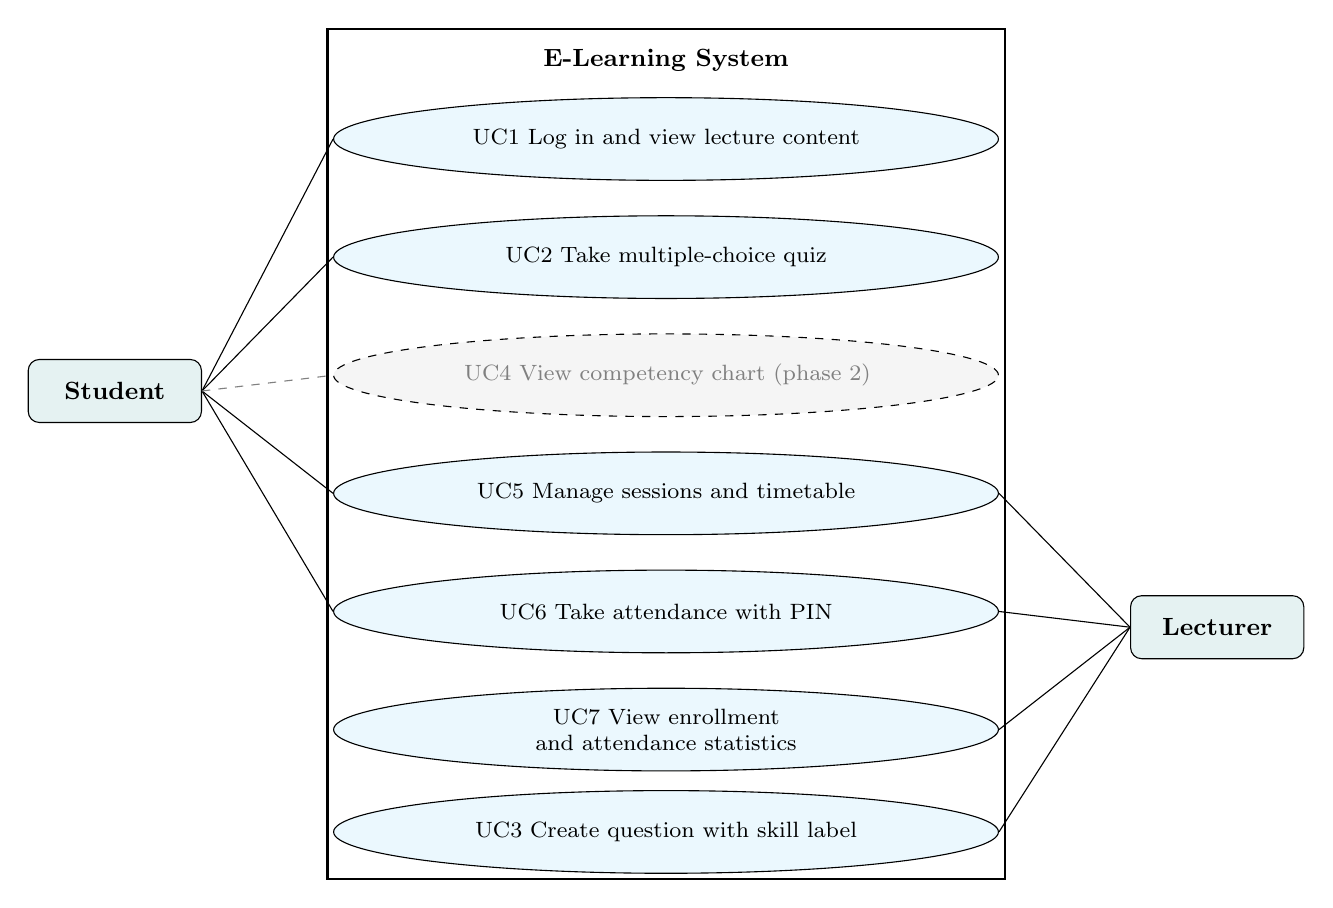
\begin{tikzpicture}[
    uc/.style={ellipse, draw, fill=cyan!8, text width=5.9cm, minimum height=1.05cm, align=center, font=\footnotesize, inner sep=1pt},
    ucp/.style={ellipse, draw, dashed, fill=gray!8, text width=5.9cm, minimum height=1.05cm, align=center, font=\footnotesize, text=gray, inner sep=1pt},
    act/.style={rectangle, draw, rounded corners, fill=teal!10, minimum width=2.2cm, minimum height=0.8cm, font=\small\bfseries, align=center},
    >=stealth]
\draw[thick] (-4.3,-9.2) rectangle (4.3,1.6);
\node[font=\small\bfseries] at (0,1.2) {E-Learning System};
\node[uc]  (u1) at (0, 0.2) {UC1 Log in and view lecture content};
\node[uc]  (u2) at (0,-1.3) {UC2 Take multiple-choice quiz};
\node[ucp] (u4) at (0,-2.8) {UC4 View competency chart (phase 2)};
\node[uc]  (u5) at (0,-4.3) {UC5 Manage sessions and timetable};
\node[uc]  (u6) at (0,-5.8) {UC6 Take attendance with PIN};
\node[uc]  (u7) at (0,-7.3) {UC7 View enrollment and attendance statistics};
\node[uc]  (u3) at (0,-8.6) {UC3 Create question with skill label};
\node[act] (st) at (-7.0,-3.0) {Student};
\node[act] (lec) at (7.0,-6.0) {Lecturer};
\foreach \u in {u1,u2,u5,u6} \draw (st.east) -- (\u.west);
\draw[dashed,gray] (st.east) -- (u4.west);
\foreach \u in {u3,u5,u6,u7} \draw (lec.west) -- (\u.east);
\end{tikzpicture}
\caption{Use case diagram of the e-learning system }
\label{fig:usecase}
\end{figure}

\subsubsection{Use Case Summary}

Table~\ref{tab:uc-summary} gives the complete list of use cases. The detailed specifications of UC5--UC7 are in Section~\ref{sec:uc-session}.

\begin{table}[H]
\centering
\caption{Use case summary}
\label{tab:uc-summary}
\begin{tblr}{colspec={Q[l,1.1cm]Q[l,3.6cm]Q[l,2.4cm]X[l]Q[l,1.8cm]}, row{1}={font=\bfseries}, hline{1,Z}={0.8pt}, hline{2}={0.4pt}, rowsep=1.5pt, rows={font=\small}}
ID & Name & Primary actor & Goal & Phase\\
UC1 & Log in and view lecture content & Student & Authenticate and open the content of a session & 1\\
UC2 & Take a multiple-choice quiz & Student & Answer questions one by one and receive immediate feedback & 1\\
UC3 & Create a question and assign a skill label & Lecturer & Add a question to the bank with a skill label & 1\\
UC4 & View competency chart & Student & See the level per skill computed from quiz history & 2\\
UC5 & Manage sessions and timetable & Lecturer (Student views) & Create and maintain the 15 sessions; view the weekly timetable & 1\\
UC6 & Take attendance with a PIN & Lecturer, Student & Open a time-limited window; students check in with a PIN & 1\\
UC7 & View enrollment and attendance statistics & Lecturer & See capacity, participation per session and rate per student & 1\\
\end{tblr}
\end{table}

\subsection{Detailed Use Case Specifications}

\subsubsection{Specifications of UC5--UC7}
\label{sec:uc-session}

UC1--UC3 are described by their main flow in Table~\ref{tab:uc-summary}; the three use cases below were added after the third meeting to cover the operation of a real class, so they are specified in full.

\begin{table}[H]
\centering
\caption{Specification of UC5 --- Manage sessions and timetable}
\label{tab:uc5}
\begin{tblr}{colspec={Q[l,3cm]X[l]}, row{1}={font=\bfseries}, hline{1,Z}={0.8pt}, hline{2}={0.4pt}, rowsep=2pt, rows={font=\small}}
Field & Content\\
Primary actor & Lecturer; secondary actors: Student (views the timetable), System\\
Description & The lecturer creates and manages the fifteen sessions of a class in the current semester (title, date, period, room). Students view the weekly timetable.\\
Trigger & The lecturer selects ``Manage sessions'' for a class, or a student opens the timetable page.\\
Pre-conditions & The user is logged in; the class (e.g.\ CO2003--CC01) exists in the active semester (e.g.\ HK261); the lecturer is in charge of the class.\\
Main flow & (1) The lecturer selects the class. (2) The system lists sessions 1--15 and a ``Create sessions'' action. (3) The lecturer chooses ``Create 15 sessions'' or adds one session. (4) The lecturer enters number, title, date, start time, end time, room (default: the default room of the class). (5) The system validates the data. (6) The system saves and confirms. (7) The system displays the weekly grid and highlights today's session. (8) A student opens the timetable, selects a week and sees the sessions of the classes he or she is enrolled in; a click shows the details and materials.\\
Alternative flows & A1 Edit a session (re-validate and save). A2 Delete a session after confirmation; related attendance and quiz data are removed by \texttt{ON DELETE CASCADE}. A3 Switch the week or switch between grid and list view.\\
Exception flows & E1 Room or time conflict: error, choose again. E2 Invalid data (missing field, date outside the semester, end not after start). E3 No permission (not the lecturer of the class). E4 System error: data are kept in the form for retry.\\
Business rules & BR1 Each class has exactly 15 sessions numbered 1--15, unique. BR2 Each session owns its materials, attendance and quiz.\\
Post-conditions & All sessions are stored in \code{course_sessions}; the timetable shows them correctly.\\
\end{tblr}
\end{table}

\begin{table}[H]
\centering
\caption{Specification of UC6 --- Take attendance with a PIN}
\label{tab:uc6}
\begin{tblr}{colspec={Q[l,3cm]X[l]}, row{1}={font=\bfseries}, hline{1,Z}={0.8pt}, hline{2}={0.4pt}, rowsep=2pt, rows={font=\small}}
Field & Content\\
Primary actors & Lecturer (opens the window), Student (checks in); secondary actor: System\\
Description & The lecturer opens an attendance window for a session; the system generates a random four-digit PIN valid for 10--15 minutes. A student who enters the correct PIN while the window is open is recorded as present. When the time runs out, the window locks automatically.\\
Trigger & The lecturer clicks ``Open attendance'' on the session page.\\
Pre-conditions & Lecturer and students are logged in; the session belongs to the lecturer's class; the student's enrollment status is ``enrolled''.\\
Main flow & (1) The lecturer clicks ``Open attendance''. (2) The system generates the PIN, sets \code{is_attendance_open = true} and computes \code{attendance_expires_at}. (3) The system shows the PIN in large type (for a projector) with a countdown and the class list. (4) A student enters the PIN on a phone or laptop. (5) The system checks that the window is open and not expired, the PIN is correct, the student belongs to the class and has not already checked in. (6) The system records status \emph{present}, method \emph{pin}, and the check-in time. (7) The lecturer's list updates. (8) At expiry the system locks the window; students without a record are shown as absent.\\
Alternative flows & A1 Manual attendance by the lecturer (present, absent, late, excused) with an optional note. A2 Close early. A3 Regenerate the PIN if it leaked; the expiry is reset.\\
Exception flows & E1 Wrong PIN: error; consecutive failures are limited. E2 Window closed or expired: nothing is recorded. E3 Already checked in: no duplicate. E4 Student not in class: rejected. E5 Connection lost: the student can retry while the window is valid.\\
Business rules & BR1 PIN = 4 random digits, valid 10--15 minutes. BR2 One attendance record per student per session. BR3 Only the lecturer of the class can open, close and edit attendance.\\
Post-conditions & Every successful check-in has a record with status \emph{present}, method \emph{pin} and a time; the window is locked after expiry or closing.\\
\end{tblr}
\end{table}

\begin{table}[H]
\centering
\caption{Specification of UC7 --- View enrollment and attendance statistics}
\label{tab:uc7}
\begin{tblr}{colspec={Q[l,3cm]X[l]}, row{1}={font=\bfseries}, hline{1,Z}={0.8pt}, hline{2}={0.4pt}, rowsep=2pt, rows={font=\small}}
Field & Content\\
Primary actor & Lecturer; secondary actor: System\\
Description & The lecturer views, for a class: enrolled students against capacity, the average attendance rate, the participation rate of each of the fifteen sessions and the attendance rate of each student.\\
Trigger & The lecturer selects ``Class statistics''.\\
Pre-conditions & The lecturer is logged in and in charge of the class; the class has enrollments; at least one session has taken place (otherwise only enrollment is shown).\\
Main flow & (1) The lecturer opens ``Class statistics''. (2) The system shows enrolled/capacity (e.g.\ 45/60) and the number of dropped students. (3) The system shows the average attendance rate. (4) The system draws a bar chart of participation for sessions 1--15. (5) The system shows a per-student table: present, absent, late, excused, percentage. (6) The lecturer clicks a bar to see the details of the session.\\
Alternative flows & A1 Filter by semester, class or range of sessions. A2 Sort by rate; highlight students under the threshold (e.g.\ 80\%). A3 Export the table to a file (if supported).\\
Exception flows & E1 No attendance yet: show enrollment and the message ``No session has been recorded yet''. E2 No student in the class. E3 No permission. E4 System error with reload.\\
Business rules & BR1 Attendance rate = (present + late) / sessions held $\times$ 100\%; excused sessions are removed from the denominator. BR2 Only students with status \emph{enrolled} are counted.\\
Post-conditions & The system does not change any data.\\
\end{tblr}
\end{table}

\subsection{Business Rules}

Table~\ref{tab:br} collects the business rules that cut across use cases and states where each one is enforced.

\begin{table}[H]
\centering
\caption{Cross-cutting business rules and enforcement points}
\label{tab:br}
\begin{tblr}{colspec={Q[l,1.2cm]X[l]X[l]}, row{1}={font=\bfseries}, hline{1,Z}={0.8pt}, hline{2}={0.4pt}, rowsep=1.5pt, rows={font=\small}}
ID & Rule & Enforced by\\
R1 & At most one semester is active at a time. & Partial unique index on \code{semesters(is_active)}\\
R2 & A class code is unique within a semester. & \code{UNIQUE (semester_id, class_code)}\\
R3 & A student has at most one enrollment row per class; a dropped student can re-enroll. & \code{UNIQUE (class_id, user_id)} and status column\\
R4 & Enrollment never exceeds the capacity. & Trigger with \texttt{FOR UPDATE}\\
R5 & Session numbers are 1--15 and unique within a class. & \code{CHECK} and \code{UNIQUE (class_id, session_number)}\\
R6 & A session ends after it starts. & \code{CHECK (end_time > start_time)}\\
R7 & A PIN has exactly four digits; the window is open if and only if a PIN and an expiry exist. & Two \code{CHECK} constraints\\
R8 & One attendance record per student per session; present and late records have a time and a method. & \code{UNIQUE (session_id, user_id)} and \code{CHECK}\\
R9 & Five failed PIN attempts in 15 minutes block the student for that session. & Table \code{attendance_pin_attempts} and application logic\\
R10 & A question has one skill, and an interaction cannot carry a different skill from its question. & Composite foreign key \code{(question_id, skill_id)}\\
\end{tblr}
\end{table}

\section{System Design}
\label{ch:design}

This section explains how the requirements of Section~\ref{ch:req} are turned into a design. It describes the methodology followed by the team, the overall pipeline of the data, the architecture, the relational schema (including the entity-relationship diagram), the API and the security design.

\subsection{Methodology}
\label{sec:method}

\subsubsection{Development Process}

The team follows an incremental process with iterations that end at a meeting with the supervisor, an approach inspired by agile development~\cite{beck2001agile, sommerville2016software}. Each iteration has five steps: (1) collect or refine requirements; (2) update the use cases and the schema; (3) implement the API and the interface; (4) test the main flows by hand and with scripted calls; (5) demonstrate to the supervisor and incorporate feedback. Table~\ref{tab:iterations} shows how the iterations so far changed the design.

\begin{table}[H]
\centering
\caption{Iterations of the project and the main design decisions}
\label{tab:iterations}
\begin{tblr}{colspec={Q[l,2.4cm]X[l]X[l]}, row{1}={font=\bfseries}, hline{1,Z}={0.8pt}, hline{2}={0.4pt}, rowsep=1.5pt, rows={font=\small}}
Iteration & Input & Main decisions and results\\
Meetings 1--2 & Project outline; survey of background material & Three-tier architecture; PostgreSQL; Next.js and Express with TypeScript; roles student, instructor, admin\\
Meeting 3 & Supervisor: the system must be a complete university LMS first & Add semesters, course classes, enrollments, 15 sessions, session materials, PIN attendance (UC5--UC7); database schema with 14 tables\\
Meeting 4 & Prototype review & BKeL-style interface; login page separating the lecturer and student roles; pilot course CO2003; statistics page\\
\end{tblr}
\end{table}

\subsubsection{Design Method for the Database}

The schema was designed in four steps: (1) identify entities and relationships from the use cases and the vocabulary of the university (semester, course, class, session, enrollment); (2) draw the ERD using the Chen notation as the conceptual reference~\cite{chen1976entity}; (3) map it to relations and normalize to 3NF~\cite{codd1970relational, silberschatz2019database}; (4) add constraints, indexes and triggers that enforce the business rules of Table~\ref{tab:br}. The result is checked by writing the queries of every use case before implementing the API.

\subsubsection{Design Method for the Interface}

The interface was designed from the BKeL screens that students know. A set of design tokens (colors, spacing, radius, shadows, font sizes) was defined first; components (card, tab, table, modal, toast, icon) are built from the tokens. This gives a consistent look and makes the dark theme a matter of redefining variables. The heuristics of~\cite{nielsen1993usability} are used as a checklist in design reviews.

\subsection{Overall Pipeline}
\label{sec:pipeline}

The ``pipeline'' of the system is the path that data follow from the moment a lecturer prepares a class until the lecturer reads the statistics at the end of the semester. Figure~\ref{fig:pipeline} shows the five stages.

\begin{figure}[H]
\centering
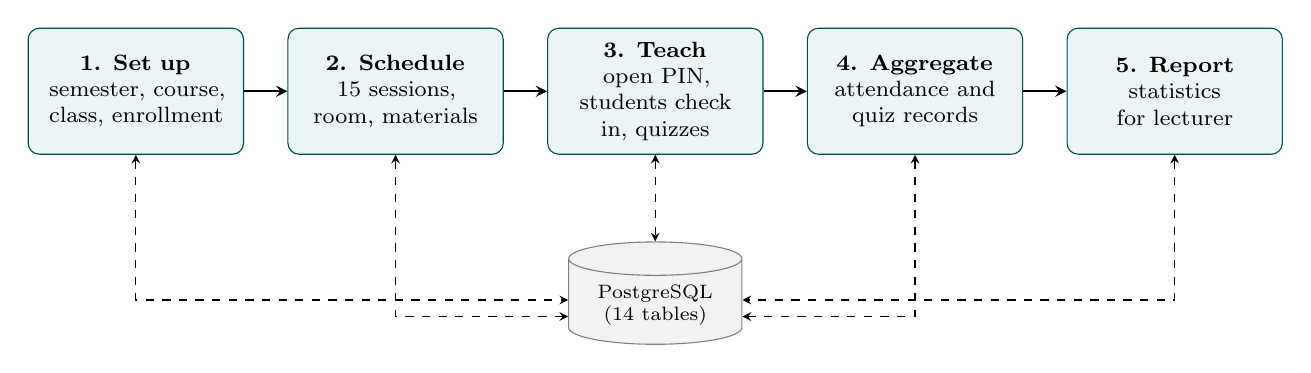
\begin{tikzpicture}[
    stage/.style={rectangle, rounded corners=4pt, draw=teal!60!black, fill=teal!8, minimum width=2.7cm, minimum height=1.6cm, align=center, font=\footnotesize, text width=2.5cm},
    data/.style={cylinder, shape border rotate=90, aspect=0.25, draw=gray, fill=gray!10, minimum height=1.3cm, minimum width=2.2cm, font=\scriptsize, align=center},
    >=stealth, node distance=0.55cm]
\node[stage] (s1) {\textbf{1. Set up}\\semester, course, class, enrollment};
\node[stage, right=of s1] (s2) {\textbf{2. Schedule}\\15 sessions, room, materials};
\node[stage, right=of s2] (s3) {\textbf{3. Teach}\\open PIN, students check in, quizzes};
\node[stage, right=of s3] (s4) {\textbf{4. Aggregate}\\attendance and quiz records};
\node[stage, right=of s4] (s5) {\textbf{5. Report}\\statistics for lecturer};
\draw[->, thick] (s1) -- (s2); \draw[->, thick] (s2) -- (s3); \draw[->, thick] (s3) -- (s4); \draw[->, thick] (s4) -- (s5);
\node[data, below=1.1cm of s3] (db) {PostgreSQL\\(14 tables)};
\draw[<->, dashed] (s1.south) |- ([yshift=2pt]db.west);
\draw[<->, dashed] (s2.south) |- ([yshift=-4pt]db.west);
\draw[<->, dashed] (s3.south) -- (db.north);
\draw[<->, dashed] (s4.south) |- ([yshift=-4pt]db.east);
\draw[<->, dashed] (s5.south) |- ([yshift=2pt]db.east);
\end{tikzpicture}
\caption{Overall pipeline of the e-learning system}
\label{fig:pipeline}
\end{figure}

\begin{enumerate}
    \item \textbf{Set up.} An administrator creates the semester (e.g.\ HK261), the course catalog entry (CO2003) and the class (CC01) with a capacity; students enroll.
    \item \textbf{Schedule.} The lecturer creates the 15 sessions in one transactional call and attaches materials to each session.
    \item \textbf{Teach.} During a session, the lecturer opens attendance; students check in with the PIN; students may take the quiz of the session.
    \item \textbf{Aggregate.} Every check-in becomes a row in \code{attendance_records}; every answer becomes a row in \code{quiz_interactions}. Rows are append-only in normal use.
    \item \textbf{Report.} The statistics endpoint aggregates the rows into enrollment, participation and rates.
\end{enumerate}

\subsection{System Architecture}
\label{sec:arch}

\subsubsection{Three-Tier Architecture}

Figure~\ref{fig:arch} shows the architecture. The browser runs the Next.js application; it talks to the REST API over HTTPS with JSON payloads; the API is the only component that talks to the database. Keeping the database behind the API is a deliberate choice for security: the client never holds database credentials, and every access goes through authentication and authorization.

\begin{figure}[H]
\centering
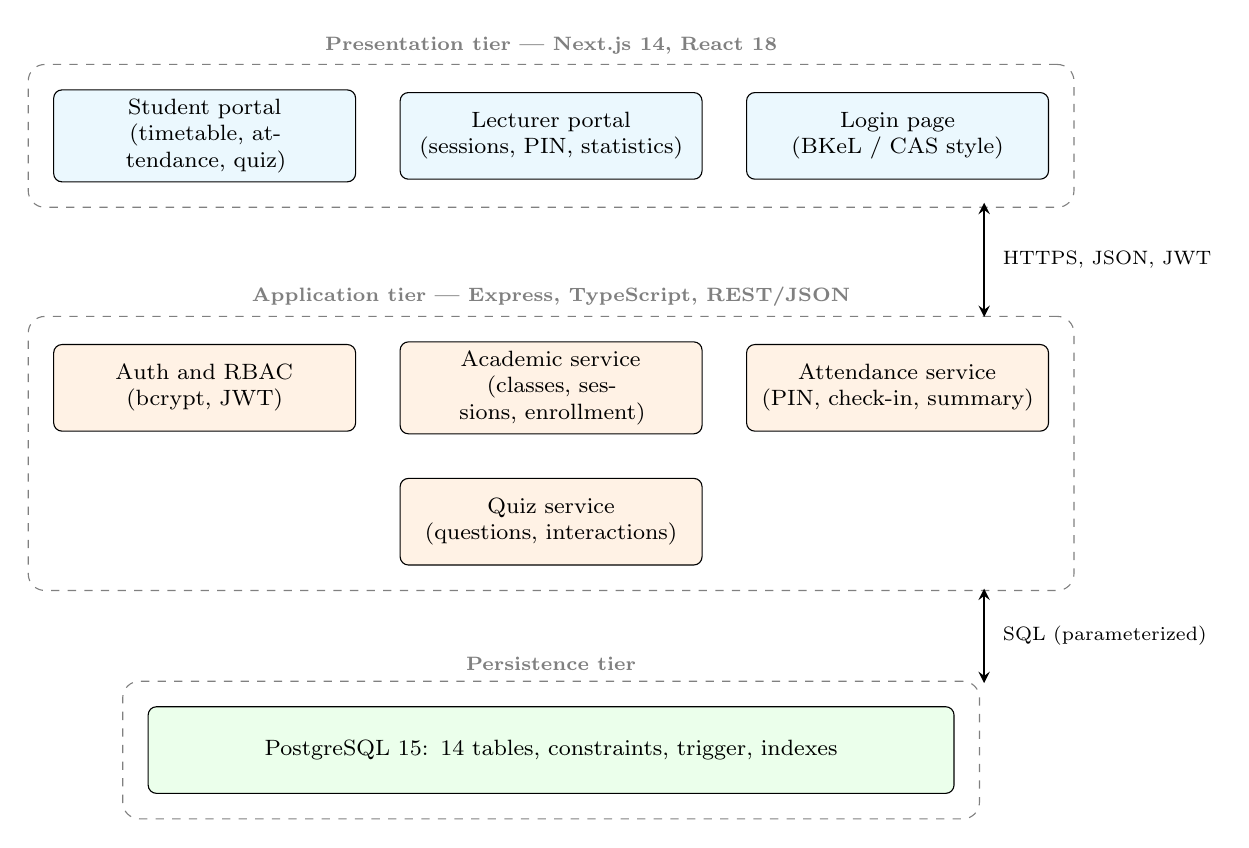
\begin{tikzpicture}[
    box/.style={rectangle, draw, rounded corners=3pt, align=center, font=\footnotesize, minimum height=1.1cm, text width=3.6cm, fill=white},
    tier/.style={rectangle, draw=gray, dashed, rounded corners=6pt, inner sep=9pt},
    >=stealth]
\node[box, fill=cyan!8] (stu) at (-4.4,2.6) {Student portal\\(timetable, attendance, quiz)};
\node[box, fill=cyan!8] (lec) at (0,2.6) {Lecturer portal\\(sessions, PIN, statistics)};
\node[box, fill=cyan!8] (log) at (4.4,2.6) {Login page\\(BKeL / CAS style)};
\node[tier, fit=(stu)(lec)(log), label={[font=\scriptsize\bfseries, gray]above:Presentation tier --- Next.js 14, React 18}] {};
\node[box, fill=orange!10] (auth) at (-4.4,-0.6) {Auth and RBAC\\(bcrypt, JWT)};
\node[box, fill=orange!10] (acad) at (0,-0.6) {Academic service\\(classes, sessions, enrollment)};
\node[box, fill=orange!10] (att) at (4.4,-0.6) {Attendance service\\(PIN, check-in, summary)};
\node[box, fill=orange!10] (quiz) at (0,-2.3) {Quiz service\\(questions, interactions)};
\node[tier, fit=(auth)(acad)(att)(quiz), label={[font=\scriptsize\bfseries, gray]above:Application tier --- Express, TypeScript, REST/JSON}] {};
\node[box, fill=green!8, text width=10cm] (db) at (0,-5.2) {PostgreSQL 15: 14 tables, constraints, trigger, indexes};
\node[tier, fit=(db), label={[font=\scriptsize\bfseries, gray]above:Persistence tier}] {};
\draw[<->, thick] (5.5,1.75) -- node[right=3pt, font=\scriptsize]{HTTPS, JSON, JWT} (5.5,0.3);
\draw[<->, thick] (5.5,-3.15) -- node[right=3pt, font=\scriptsize]{SQL (parameterized)} (5.5,-4.35);
\end{tikzpicture}
\caption{Three-tier architecture of the system}
\label{fig:arch}
\end{figure}

\subsubsection{Components and Responsibilities}

\begin{table}[H]
\centering
\caption{Components and their responsibilities}
\label{tab:components}
\begin{tblr}{colspec={Q[l,3.2cm]X[l]}, row{1}={font=\bfseries}, hline{1,Z}={0.8pt}, hline{2}={0.4pt}, rowsep=1.5pt, rows={font=\small}}
Component & Responsibility\\
Next.js application & Renders pages, keeps UI state (theme, active tab, modals), calls the API, shows feedback (toasts, countdowns).\\
Auth middleware & Verifies the JWT of every protected request and attaches the user and the role to the request.\\
Academic routes & Schedule of the current user, sessions of a class, bulk creation of the 15 sessions, enrollment.\\
Attendance routes & Open and close the window, check in with the PIN, class attendance summary.\\
Quiz routes & Return published questions without the answer key; record the interactions of a submission.\\
Expiry sweep & A timer in the server process that closes attendance windows whose expiry has passed (every 15 seconds).\\
Database & Stores data and enforces the invariants of Table~\ref{tab:br}.\\
\end{tblr}
\end{table}

\subsubsection{Sequence of the PIN Attendance}

Figure~\ref{fig:seq-att} shows the sequence of messages for UC6. The student does not need to see the PIN anywhere in the interface until the lecturer announces it in class; the API returns the PIN only to the instructor of the class (or an administrator).

\begin{figure}[H]
\centering
\resizebox{\linewidth}{!}{%
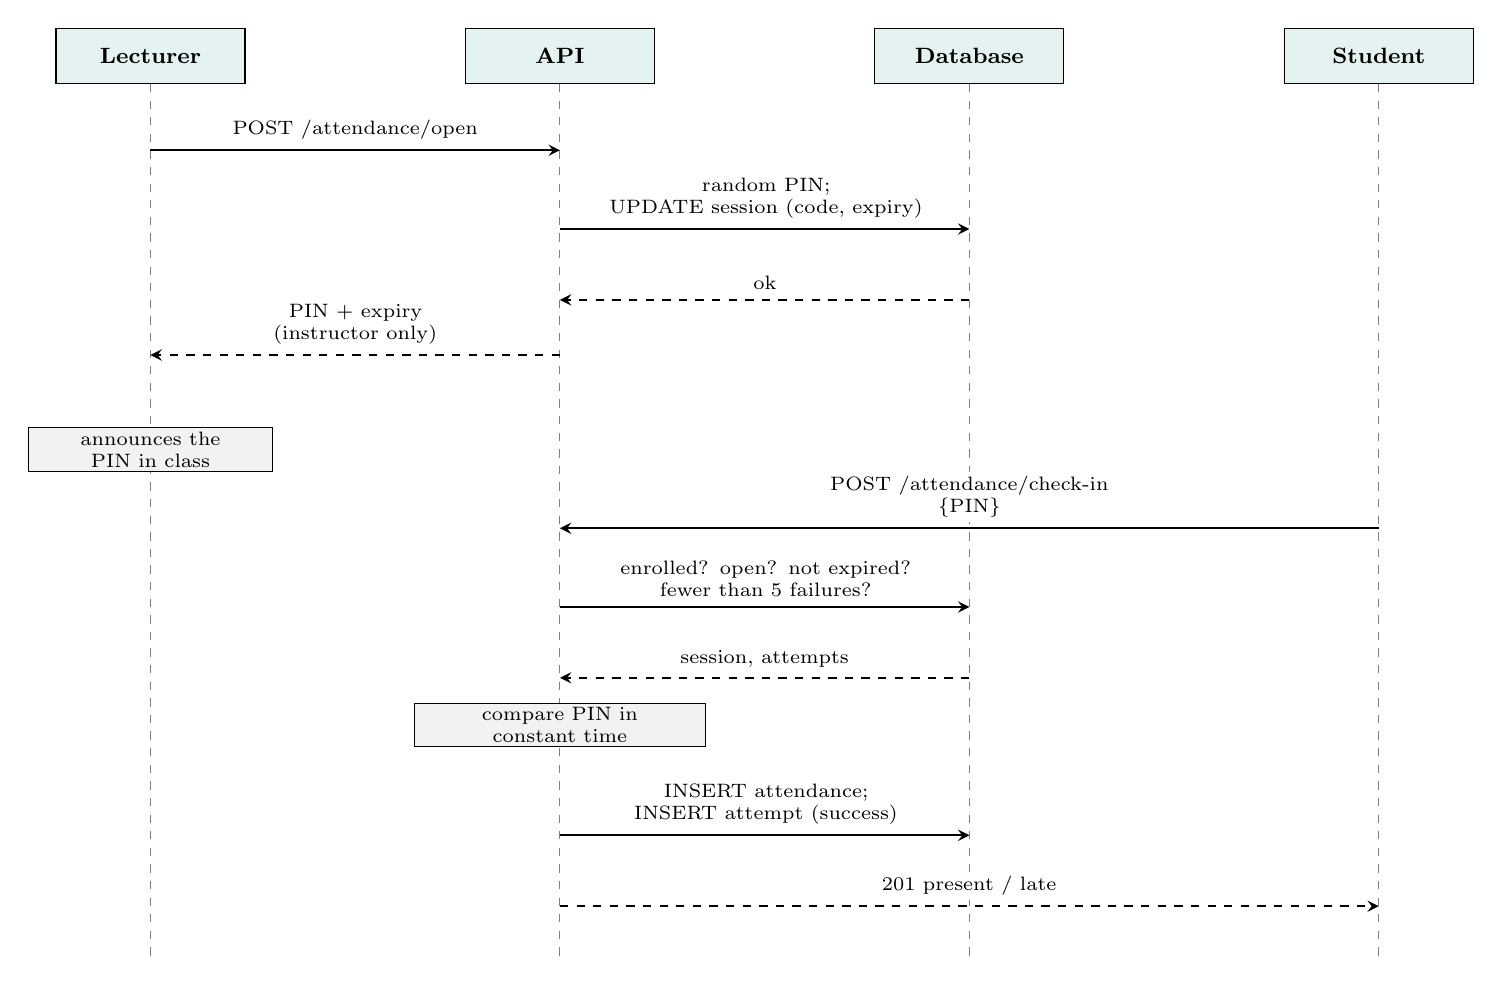
\begin{tikzpicture}[x=1.0cm,y=1.0cm,
    life/.style={dashed, gray},
    head/.style={rectangle, draw, fill=teal!10, minimum width=2.4cm, minimum height=0.7cm, font=\footnotesize\bfseries},
    msg/.style={->, >=stealth, thick},
    lab/.style={font=\scriptsize, fill=white, inner sep=1.5pt, align=center, text width=4.3cm},
    >=stealth]
\node[head] (L) at (0,0) {Lecturer};
\node[head] (A) at (5.2,0) {API};
\node[head] (D) at (10.4,0) {Database};
\node[head] (S) at (15.6,0) {Student};
\foreach \n in {L,A,D,S} \draw[life] (\n) -- ++(0,-11.5);
\draw[msg] (0,-1.2) -- node[lab, above=2pt]{POST /attendance/open} (5.2,-1.2);
\draw[msg] (5.2,-2.2) -- node[lab, above=2pt]{random PIN;\\UPDATE session (code, expiry)} (10.4,-2.2);
\draw[msg, dashed] (10.4,-3.1) -- node[lab, above=2pt]{ok} (5.2,-3.1);
\draw[msg, dashed] (5.2,-3.8) -- node[lab, above=2pt]{PIN + expiry\\(instructor only)} (0,-3.8);
\node[lab, draw, fill=gray!10, text width=3cm] at (0,-5.0) {announces the PIN in class};
\draw[msg] (15.6,-6.0) -- node[lab, above=2pt]{POST /attendance/check-in\\\{PIN\}} (5.2,-6.0);
\draw[msg] (5.2,-7.0) -- node[lab, above=2pt]{enrolled? open? not expired?\\fewer than 5 failures?} (10.4,-7.0);
\draw[msg, dashed] (10.4,-7.9) -- node[lab, above=2pt]{session, attempts} (5.2,-7.9);
\node[lab, draw, fill=gray!10, text width=3.6cm] at (5.2,-8.5) {compare PIN in constant time};
\draw[msg] (5.2,-9.9) -- node[lab, above=2pt]{INSERT attendance;\\INSERT attempt (success)} (10.4,-9.9);
\draw[msg, dashed] (5.2,-10.8) -- node[lab, above=2pt]{201 present / late} (15.6,-10.8);
\end{tikzpicture}}
\caption{Sequence diagram of the PIN attendance (UC6)}
\label{fig:seq-att}
\end{figure}

\subsubsection{State of an Attendance Window}

The window of a session is a small state machine (Figure~\ref{fig:state}). The \texttt{CHECK} constraint of the table makes the invalid combinations unrepresentable: the flag \code{is_attendance_open} is true exactly when both the code and the expiry are present.

\begin{figure}[H]
\centering
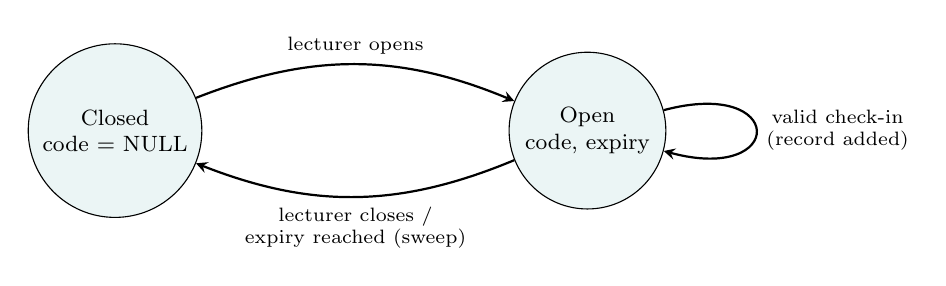
\begin{tikzpicture}[st/.style={circle, draw, fill=teal!8, minimum size=1.7cm, align=center, font=\footnotesize}, >=stealth]
\node[st] (c) at (0,0) {Closed\\code = NULL};
\node[st] (o) at (6,0) {Open\\code, expiry};
\draw[->, thick] (c) to[bend left=22] node[above, font=\scriptsize]{lecturer opens} (o);
\draw[->, thick] (o) to[bend left=22] node[below, font=\scriptsize, align=center]{lecturer closes /\\expiry reached (sweep)} (c);
\draw[->, thick] (o) to[loop right] node[right, font=\scriptsize, align=center]{valid check-in\\(record added)} (o);
\end{tikzpicture}
\caption{State of an attendance window}
\label{fig:state}
\end{figure}

\subsection{Database Design}
\label{sec:db}

\subsubsection{Entity-Relationship Diagram}

Figure~\ref{fig:erd} shows the ERD of the schema. It has fourteen tables: \code{semesters}, \code{courses}, \code{course_classes}, \code{enrollments}, \code{course_sessions}, \code{session_materials}, \code{attendance_records}, \code{attendance_pin_attempts}, \code{users}, \code{skills}, \code{quizzes}, \code{questions}, \code{quiz_interactions} and \code{schema_version}.

\begin{figure}[H]
\centering
\makebox[\textwidth][c]{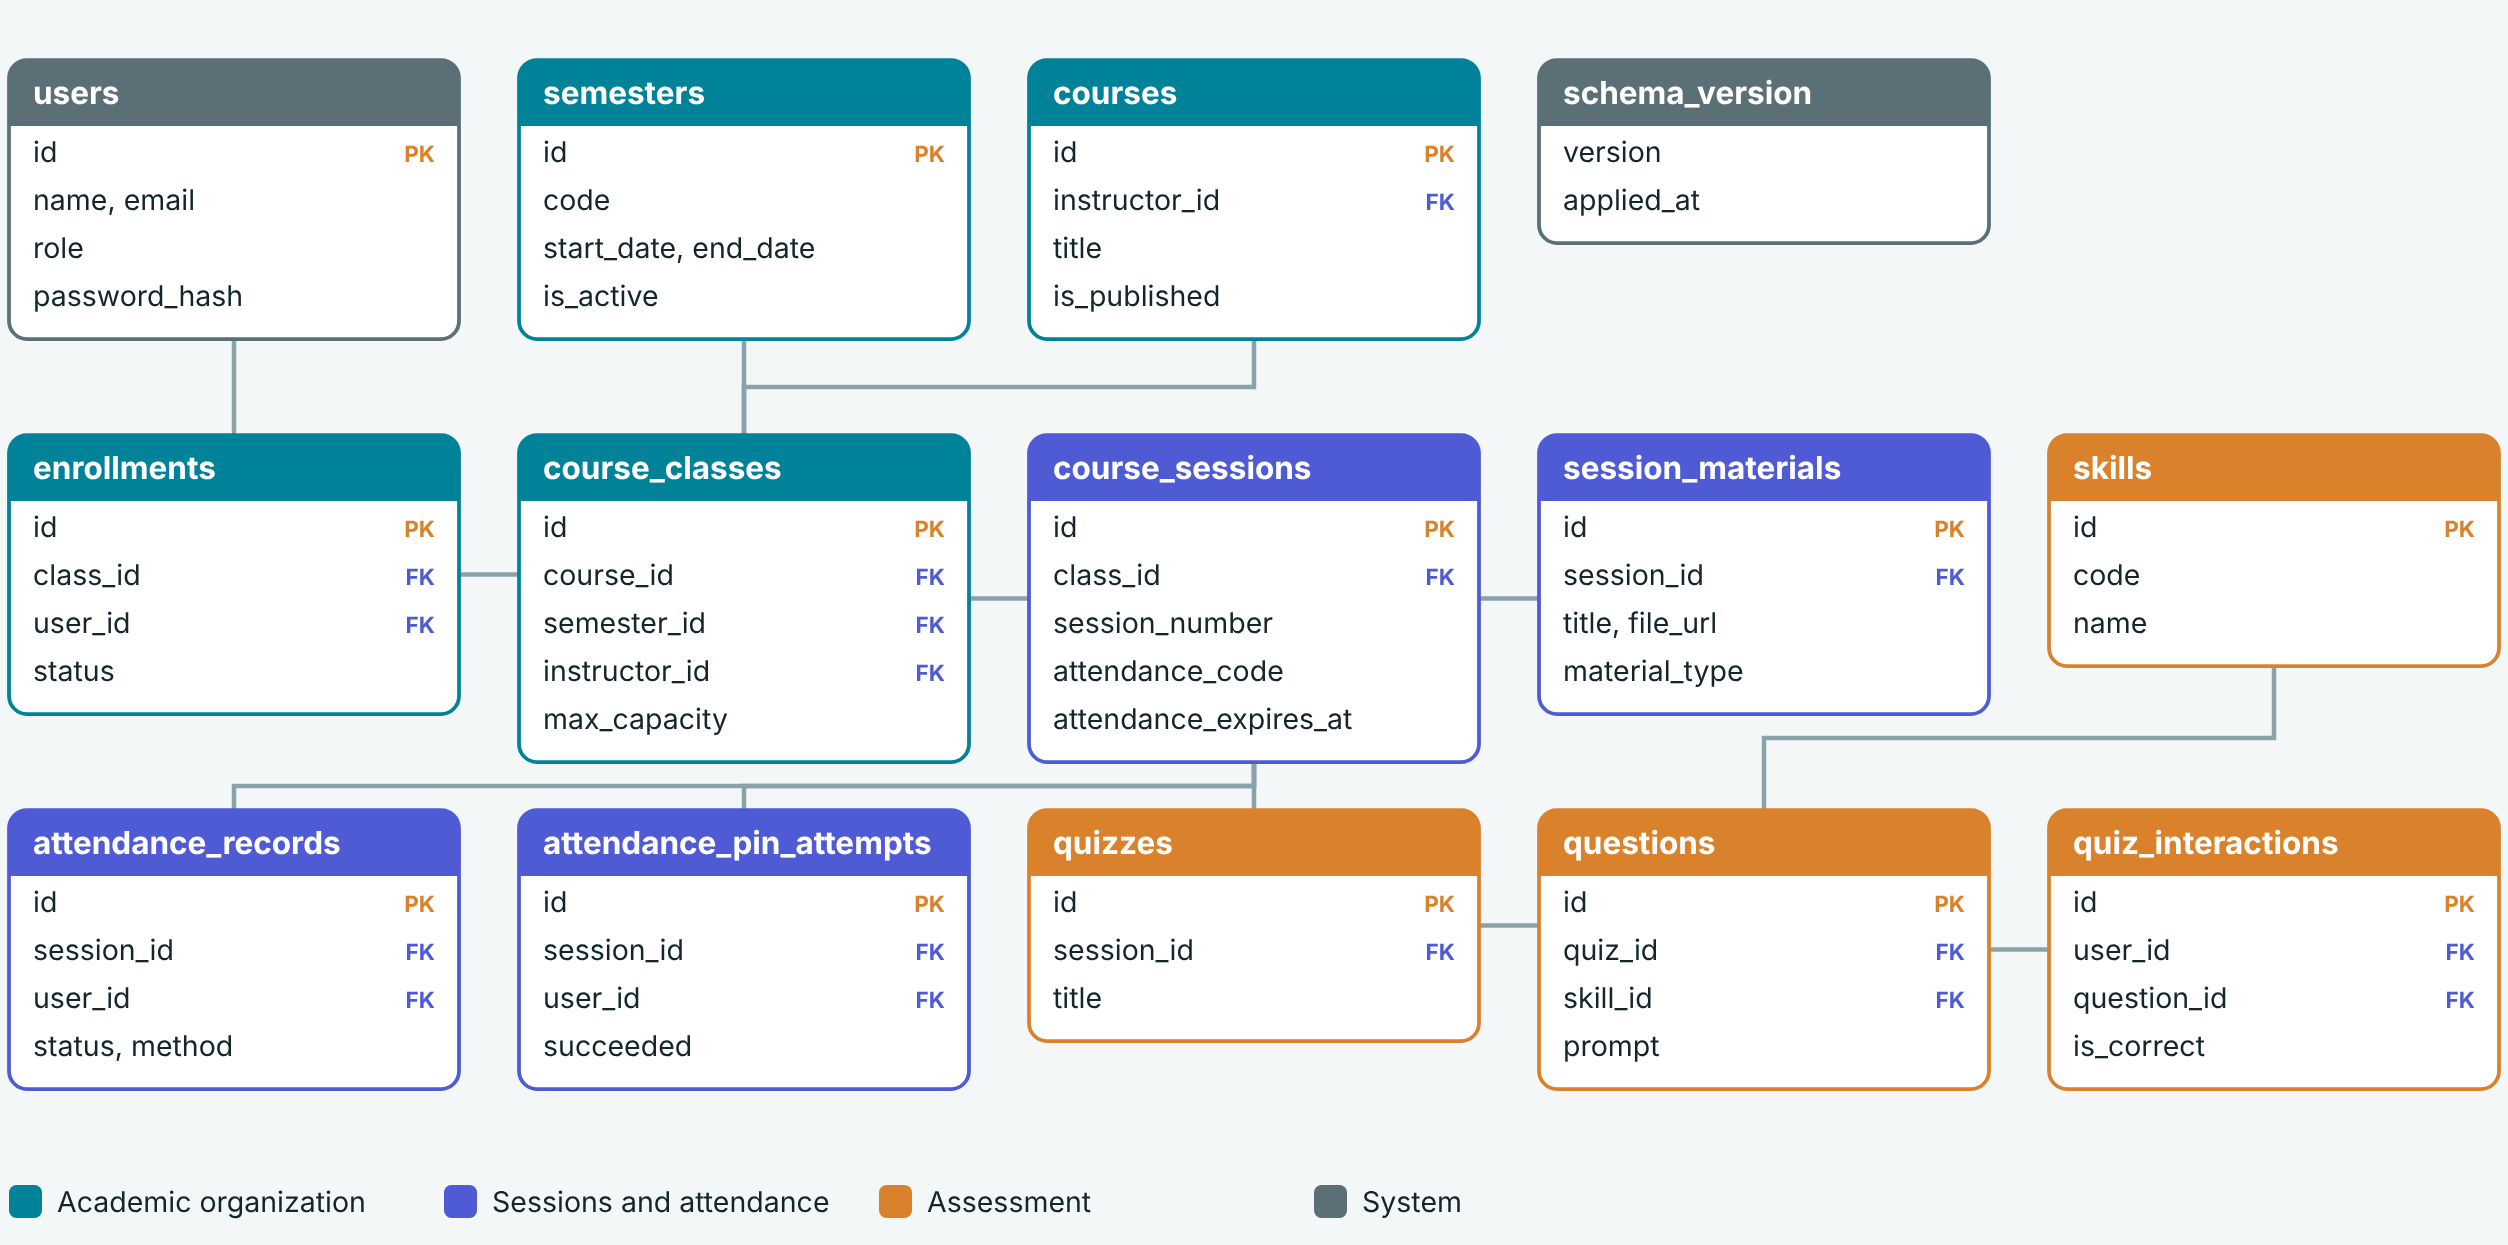
\includegraphics[width=1.18\textwidth]{images/erd.png}}
\caption{Entity-relationship diagram of the database}
\label{fig:erd}
\end{figure}

The central entity is \code{course_classes}: it is an \emph{offering} of a \code{course} in a \code{semester} taught by an instructor. Students are linked to it through \code{enrollments}. A class owns fifteen \code{course_sessions}; each session owns its \code{session_materials}, \code{attendance_records}, \code{quizzes} and \code{attendance_pin_attempts}.

\subsubsection{Data Dictionary}

Tables~\ref{tab:dict1} and~\ref{tab:dict2} summarize the tables. Primary keys are UUIDs generated by \code{gen_random_uuid()}.

\begin{table}[H]
\centering
\caption{Data dictionary (1/2): users, academic structure, schedule}
\label{tab:dict1}
\begin{tblr}{colspec={Q[l,3.3cm]X[l]}, row{1}={font=\bfseries}, hline{1,Z}={0.8pt}, hline{2}={0.4pt}, rowsep=2pt, rows={font=\small}}
Table & Main columns, constraints and meaning\\
\code{users} & \code{name}, \code{email} (unique), \code{password_hash}, \code{role} $\in$ \{student, instructor, admin\}. Self-registration creates students only.\\
\code{semesters} & \code{code} (unique, e.g.\ HK261), \code{name}, \code{start_date}, \code{end_date} with \code{CHECK (start_date <= end_date)}, \code{is_active}; a partial unique index allows at most one active semester.\\
\code{courses} & Catalog entry: \code{instructor_id} (owner), \code{title}, \code{description}, \code{is_published}.\\
\code{course_classes} & An offering: \code{course_id} (cascade), \code{semester_id} (restrict), \code{class_code}, \code{instructor_id} (restrict), \code{max_capacity > 0}, \code{default_room}. \code{UNIQUE (semester_id, class_code)}.\\
\code{enrollments} & \code{class_id}, \code{user_id}, \code{status} $\in$ \{enrolled, dropped\}, \code{enrolled_at}, \code{final_grade} in $[0,100]$. \code{UNIQUE (class_id, user_id)}. Capacity trigger.\\
\code{course_sessions} & \code{class_id}, \code{session_number} in $[1,15]$, \code{title}, \code{session_date}, \code{start_time}, \code{end_time}, \code{room}, and the attendance state: \code{attendance_code}, \code{is_attendance_open}, \code{attendance_expires_at}. \code{UNIQUE (class_id, session_number)}.\\
\code{session_materials} & \code{session_id}, \code{title}, \code{material_type} $\in$ \{slide, code, video\}, \code{file_url}, \code{position}. \code{UNIQUE (session_id, position)}.\\
\end{tblr}
\end{table}

\begin{table}[H]
\centering
\caption{Data dictionary (2/2): attendance, assessment, metadata}
\label{tab:dict2}
\begin{tblr}{colspec={Q[l,3.3cm]X[l]}, row{1}={font=\bfseries}, hline{1,Z}={0.8pt}, hline{2}={0.4pt}, rowsep=2pt, rows={font=\small}}
Table & Main columns, constraints and meaning\\
\code{attendance_records} & \code{session_id}, \code{user_id}, \code{status} $\in$ \{present, absent, late, excused\}, \code{checkin_time}, \code{method} $\in$ \{pin, qr, manual\}, \code{note}. \code{UNIQUE (session_id, user_id)}. Present or late rows must have a time and a method.\\
\code{attendance_pin_attempts} & \code{session_id}, \code{user_id}, \code{attempted_at}, \code{succeeded}. Partial index on failed attempts supports the rate-limit query.\\
\code{skills} & Knowledge component: \code{code} (unique, e.g.\ \code{DSA-LINKEDLIST}), \code{name}, \code{description}.\\
\code{quizzes} & \code{session_id} (required), \code{title}, \code{is_published}.\\
\code{questions} & \code{quiz_id}, \code{skill_id}, \code{prompt}, \code{options} (JSONB), \code{correct_answer} (private), \code{position}. \code{UNIQUE (id, skill_id)} supports the composite foreign key.\\
\code{quiz_interactions} & One row per answer: \code{user_id}, \code{session_id}, \code{question_id}, \code{skill_id}, \code{is_correct}, \code{attempt_count}, \code{created_at}. Composite foreign key \code{(question_id, skill_id)}.\\
\code{schema_version} & Installed schema version, inserted idempotently.\\
\end{tblr}
\end{table}

\subsubsection{Normalization}
\label{sec:normalization}

All tables are in 3NF: each non-key attribute depends on the key only. Examples of design decisions are:

\begin{itemize}
    \item The capacity and the default room belong to the \emph{class}, not to the course, because the same course can be offered with different capacities in different semesters. They are therefore columns of \code{course_classes}.
    \item The enrollment is a separate relation because a student has many classes and a class has many students (many-to-many); \code{status} and \code{final_grade} depend on the pair (class, student).
    \item The skill is stored once in \code{skills}, and \code{questions} refers to it. The redundant \code{skill_id} in \code{quiz_interactions} is a \emph{deliberate} denormalization: it keeps the history of what skill a response was about, and the composite foreign key guarantees that it never differs from the skill of the question.
    \item The attendance state of the current window (\code{attendance_code}, \code{is_attendance_open}, \code{attendance_expires_at}) is stored in \code{course_sessions} because it is a transient attribute of exactly one session and there is at most one active window per session.
\end{itemize}

\subsubsection{Integrity Mechanisms}

\paragraph{Capacity trigger.} Listing~\ref{lst:trigger} shows the trigger function. The statement \texttt{SELECT ... FOR UPDATE} locks the class row, so two concurrent enrollments into the same class are processed one after the other; the second one sees the first. This prevents the anomaly described in Section~\ref{sec:method}~\cite{berenson1995critique, bernstein1981concurrency, postgresdocs}.

\begin{lstlisting}[language=SQLpg, caption={Capacity enforcement trigger (excerpt of \texttt{schema.sql})}, label={lst:trigger}]
CREATE OR REPLACE FUNCTION enforce_course_class_capacity() RETURNS trigger AS $$
DECLARE
  capacity_limit INTEGER;
  current_enrollment_count INTEGER;
BEGIN
  IF NEW.status <> 'enrolled' THEN
    RETURN NEW;
  END IF;
  -- Serialize joins to the same class
  SELECT max_capacity INTO capacity_limit
  FROM course_classes WHERE id = NEW.class_id FOR UPDATE;

  SELECT count(*) INTO current_enrollment_count
  FROM enrollments
  WHERE class_id = NEW.class_id AND status = 'enrolled'
    AND (TG_OP = 'INSERT' OR id <> NEW.id);

  IF current_enrollment_count >= capacity_limit THEN
    RAISE EXCEPTION 'Class capacity has been reached' USING ERRCODE = '23514';
  END IF;
  RETURN NEW;
END;
$$ LANGUAGE plpgsql;
\end{lstlisting}

\paragraph{Window consistency.} Listing~\ref{lst:check} shows the constraints that make an inconsistent attendance state impossible.

\begin{lstlisting}[language=SQLpg, caption={Constraints of \texttt{course\_sessions}}, label={lst:check}]
CHECK (end_time > start_time),
CHECK (attendance_code IS NULL OR attendance_code ~ '^[0-9]{4}$'),
CHECK (is_attendance_open =
       (attendance_code IS NOT NULL AND attendance_expires_at IS NOT NULL))
\end{lstlisting}

\paragraph{Delete behavior.} Deleting a class cascades to its sessions, and from there to materials, attendance, quizzes, interactions and attempts. Deleting a semester or an instructor who still has classes is \emph{restricted}, which protects active offerings from accidental removal. Deleting a skill that is used by a question is restricted.

\subsubsection{Indexes}

The indexes support the queries of the use cases: sessions of a class ordered by date (UC5); enrollments counted by class and status (capacity, UC7); attendance lookup by (user, session); failed PIN attempts of a student in a window (UC6); and interactions by user, skill and time (quiz history).

\subsection{API Design}
\label{sec:api}

Table~\ref{tab:api} lists the endpoints. All endpoints other than registration and login require a valid JWT. Errors use standard HTTP status codes~\cite{rfc9110}; too many failed PIN attempts return 429~\cite{rfc6585}.

\begin{table}[H]
\centering
\caption{REST endpoints of the back end}
\label{tab:api}
\begin{tblr}{colspec={Q[l,1.3cm]Q[l,6.1cm]X[l]}, row{1}={font=\bfseries}, hline{1,Z}={0.8pt}, hline{2}={0.4pt}, rowsep=2pt, rows={font=\small}}
Method & Path & Purpose and access\\
POST & \code{/api/auth/register} & Create a student account\\
POST & \code{/api/auth/login} & Return a one-day JWT\\
GET & \code{/api/schedule?semesterId=} & Sessions of the current user (enrolled or taught), ordered by date and time\\
GET & \code{/api/classes/:classId/sessions} & Sessions and materials of a class; the PIN is visible only to its instructor or an administrator while active\\
POST & \code{/api/classes/:classId/enroll} & Student enrollment; the trigger serializes concurrent joins\\
POST & \code{/api/classes/:classId/sessions} & Instructor creates one session\\
POST & \code{/api/classes/:classId/sessions/bulk} & Instructor creates sessions 1--15 in one transaction\\
POST & \code{/api/sessions/:id/attendance/open} & Open the window for 10--15 minutes (default 10); returns PIN and expiry\\
POST & \code{/api/sessions/:id/attendance/close} & Close the window and clear the PIN\\
POST & \code{/api/sessions/:id/attendance/check-in} & Enrolled student submits \texttt{\{attendanceCode\}}\\
GET & \code{/api/classes/:classId/attendance/summary} & Capacity, enrolled, completed sessions, overall rate, rate per student\\
GET & \code{/api/sessions/:id/quizzes} & Published questions of a session, without the answer key\\
POST & \code{/api/quizzes/:quizId/submit} & Record correctness, skill, attempt and session per question\\
\end{tblr}
\end{table}

\subsection{Security Design}
\label{sec:pin-security}

\subsubsection{Threat Model}

The assets are the integrity of attendance data, the confidentiality of the answer key and the credentials of users. We consider the following threats, which follow the common web risks of~\cite{owasptop10} and the verification requirements of~\cite{owaspasvs}:

\begin{itemize}
    \item a student tries to check in without being in the room (proxy attendance);
    \item a student guesses the PIN by repeated requests;
    \item a user calls an endpoint of a role he or she does not have;
    \item a student reads the answer key from a quiz response;
    \item SQL injection through a request parameter;
    \item two requests race to take the last seat of a class.
\end{itemize}

\subsubsection{Countermeasures}

\begin{table}[H]
\centering
\caption{Threats and countermeasures}
\label{tab:threats}
\begin{tblr}{colspec={Q[l,3.6cm]X[l]}, row{1}={font=\bfseries}, hline{1,Z}={0.8pt}, hline{2}={0.4pt}, rowsep=1.5pt, rows={font=\small}}
Threat & Countermeasure\\
Proxy attendance & The PIN is shown only on the lecturer's screen and expires in 10--15 minutes; a sweep every 15 seconds and a check at check-in both enforce the expiry.\\
PIN guessing & Five failed attempts per student and session in 15 minutes lead to HTTP 429; only enrolled students can try; every attempt is logged in \code{attendance_pin_attempts}; a transaction-level advisory lock on (session, student) serializes parallel requests of the same student so that concurrent guesses cannot bypass the counter.\\
Timing side channel & The submitted PIN is compared with \code{timingSafeEqual} from the Node.js \code{crypto} module, which takes the same time whatever the content.\\
Weak PIN generation & PINs come from \code{randomInt} of \code{node:crypto}, a cryptographically secure generator, not from \code{Math.random}.\\
Privilege escalation & The JWT carries the role; each route checks it; opening and closing attendance and reading the PIN require the instructor of that class or an administrator.\\
Answer-key leakage & The quiz endpoint selects columns explicitly and never returns \code{correct_answer}.\\
Credential theft & bcrypt hashes~\cite{provos1999bcrypt}; JWT with a long private secret read from the environment; tokens expire after one day.\\
SQL injection & Parameterized queries only.\\
Enrollment race & Row lock in the trigger (Listing~\ref{lst:trigger}).\\
\end{tblr}
\end{table}

\subsubsection{Residual Risk of the PIN}

With 10\,000 possible PINs and a limit of five failed attempts in a window, a single student who guesses distinct values has a probability of at most $5/10\,000 = 0.05\%$ of finding the PIN before being blocked. If $k$ students cooperate and each makes five distinct guesses, the probability grows to at most $5k/10\,000$; for $k=10$ it is 0.5\%. The mechanism does not protect against a student who \emph{receives the PIN from a classmate who is present}; no PIN scheme can, and this is why the validity is kept short. For a stronger guarantee the system could add a second factor in the future, for example a one-time code that rotates every minute (Section~\ref{ch:plan}).

\section{Implementation and Prototype}
\label{ch:impl}

This section describes how the design was implemented: the project structure, the back end, the front end and its design system, the pilot dataset, and the traceability from requirements to code.

\subsection{Project Structure and Environment}

The source code is hosted in one Git repository~\cite{chacon2014progit} with three main folders: \code{frontend} (Next.js application), \code{backend} (Express API and SQL schema) and \code{docs} (diagrams, use cases, data dictionary, pilot dataset). Table~\ref{tab:stack} gives the versions and roles of the main tools.

\begin{table}[H]
\centering
\caption{Technology stack and versions}
\label{tab:stack}
\begin{tblr}{colspec={Q[l,3.4cm]Q[l,3.4cm]X[l]}, row{1}={font=\bfseries}, hline{1,Z}={0.8pt}, hline{2}={0.4pt}, rowsep=3pt}
Layer & Technology & Role\\
Front end & Next.js 14.2, React 18.3 & Pages, components, client-side state~\cite{nextjsdocs, reactdocs}\\
Styling & Plain CSS with custom properties & Design tokens, light and dark themes\\
Back end & Node.js, Express 5, TypeScript & REST API~\cite{nodedocs, expressdocs, typescriptdocs}\\
Security libraries & \texttt{bcryptjs}, \texttt{jsonwebtoken} & Password hashing and tokens~\cite{provos1999bcrypt, rfc7519}\\
Database driver & \texttt{pg} & Parameterized SQL\\
Database & PostgreSQL 15, \texttt{pgcrypto} & Storage and integrity~\cite{postgresdocs}\\
Version control & Git & Collaboration of three developers\\
\end{tblr}
\end{table}

\subsection{Back-End Implementation}

\subsubsection{Structure}

The API is organized in the following modules:

\begin{itemize}
    \item \code{config/}: reads environment variables (database URL, JWT secret, port) and creates the connection pool;
    \item \code{middleware/auth.ts}: verifies the JWT and provides \code{requireRoles(...)};
    \item \code{routes/auth.ts} and \code{routes/quizzes.ts}: registration, login and quiz submission;
    \item \code{routes/academic.ts}: schedule, sessions, enrollment, attendance and statistics;
    \item \code{server.ts}: starts the HTTP server and the expiry sweep.
\end{itemize}

\subsubsection{Authentication and Roles}

Registration hashes the password with bcrypt and inserts a student. Login verifies the hash and returns a JWT valid for one day containing the user identifier and role. The middleware \code{requireRoles} receives the list of allowed roles of a route; for example, the opening of attendance is restricted to \code{instructor} and \code{admin}, and the route additionally checks that the instructor owns the class.

\subsubsection{Bulk Creation of Sessions}

The endpoint \code{POST /api/classes/:classId/sessions/bulk} creates sessions 1--15 inside one database transaction. If one session is invalid (for example, its end time is before its start time) the whole request is rolled back, so a class never ends up with a partial timetable. This follows the business rule that a class has exactly fifteen sessions (R5 in Table~\ref{tab:br}).

\subsubsection{PIN Attendance}

Opening the window generates the PIN and the expiry:

\begin{lstlisting}[language=TS, caption={Generation of the PIN (excerpt)}, label={lst:pin}]
import { randomInt, timingSafeEqual } from 'node:crypto'

// 0000 - 9999, uniformly distributed, from a cryptographically secure source
const code = randomInt(0, 10_000).toString().padStart(4, '0')
\end{lstlisting}

The check-in endpoint runs in one transaction and follows the steps below. The listing shows the order of the checks; the HTTP status code of each rejection is given in Table~\ref{tab:checkin}.

\begin{enumerate}
    \item Load the session and verify that the student has an \emph{enrolled} row for its class.
    \item If the window is closed or the expiry has passed, clear the PIN and answer \texttt{410}.
    \item Take a transaction-level advisory lock on the pair (session, student) so that parallel requests of the same student are processed one at a time.
    \item Count the failed attempts of the student for this session in the last 15 minutes; if there are five or more, answer \texttt{429}.
    \item Compare the PIN with \code{timingSafeEqual}. If different, insert a failed attempt and answer \texttt{401}.
    \item Insert the attendance record with \code{ON CONFLICT (session_id, user_id) DO NOTHING}. If nothing was inserted, answer \texttt{409}; otherwise log a successful attempt and answer \texttt{201}.
\end{enumerate}

\begin{table}[H]
\centering
\caption{Outcomes of the check-in endpoint}
\label{tab:checkin}
\begin{tblr}{colspec={Q[l,1.6cm]X[l]}, row{1}={font=\bfseries}, hline{1,Z}={0.8pt}, hline{2}={0.4pt}, rowsep=3pt}
Status & Meaning\\
201 & Check-in recorded. The status is \emph{late} if the check-in time is after the scheduled start of the session in the Asia/Ho\_Chi\_Minh time zone, and \emph{present} otherwise.\\
401 & The PIN is incorrect; a failed attempt is logged.\\
409 & The student already has a record for this session.\\
410 & The window is closed or expired.\\
429 & Five failed attempts in the last 15 minutes.\\
\end{tblr}
\end{table}

A timer started with the server calls a function every 15 seconds that sets \code{attendance_code}, \code{is_attendance_open} and \code{attendance_expires_at} to their closed values for every session whose expiry has passed. The check-in endpoint also tests the expiry itself, so the correctness of the system does not rely on the timer.

\subsubsection{Attendance Rate}

The summary endpoint computes, for each student, the number of attended sessions among the completed ones. A session is \emph{completed} when its scheduled end time (in the Asia/Ho\_Chi\_Minh time zone) has passed. Present and late count as attended, excused sessions are removed from the denominator, and a missing record counts as not attended. The overall rate is the number of attended check-ins divided by the number of expected student--session pairs without excused ones.

\subsubsection{Quiz Submission}

\code{POST /api/quizzes/:quizId/submit} receives the list of answers, loads the answer key on the server, compares, and inserts one \code{quiz_interactions} row per answer with the question, skill, session, correctness and attempt number. The learner-facing quiz endpoint never selects \code{correct_answer}.

\subsection{Front-End Implementation}

\subsubsection{Design System}

The interface is a reproduction of the BKeL portal with a refined design system:

\begin{itemize}
    \item \textbf{Color.} Primary \texttt{\#008299} (BKeL teal) and a neutral scale; semantic colors for present, late, absent and excused. Both themes keep a contrast ratio of at least 4.5:1 for body text.
    \item \textbf{Icons.} 100\% inline SVG in the Moodle style for activity types (PDF, quiz, attendance, code, forum, calendar, timetable). No emoji is used anywhere.
    \item \textbf{Course cards.} Geometric vector patterns (circles, triangles) similar to the Moodle default course images.
    \item \textbf{Motion.} Short transitions (under 400\,ms) for tab changes and modals; the reduced-motion setting of the operating system is respected.
    \item \textbf{Themes.} Light and dark themes by switching CSS variables; the choice is stored in the browser.
\end{itemize}

\subsubsection{Pages}

Table~\ref{tab:pages} lists the pages and tabs of the prototype.

\begin{table}[H]
\centering
\caption{Pages and tabs of the front-end prototype}
\label{tab:pages}
\begin{tblr}{colspec={Q[l,3.4cm]X[l]Q[l,2.4cm]}, row{1}={font=\bfseries}, hline{1,Z}={0.8pt}, hline{2}={0.4pt}, rowsep=3pt}
Page or tab & Content & Use case\\
Login (CAS style) & Separate entry for the lecturer and the student role; sample accounts for demonstration & UC1\\
Home / dashboard / my courses & Course cards for the active semester & UC1\\
Course: Sessions & The 15 sessions with title, date, room and materials & UC5\\
Course: Attendance & Open window with PIN and countdown (lecturer); PIN entry (student); live list & UC6\\
Course: Timetable & Weekly grid with today's session highlighted & UC5\\
Course: Participants & Enrolled students & UC7\\
Course: Statistics & Enrollment against capacity; participation per session; rate per student & UC7\\
Course: Quiz & Question bank of 40 questions; whole-bank quiz or one quiz per session & UC2\\
\end{tblr}
\end{table}

\subsubsection{Screens}

Figures~\ref{fig:login}--\ref{fig:stats} show the main screens. The interface language of the prototype is Vietnamese, in agreement with the users of HCMUT.

\begin{figure}[H]
\centering
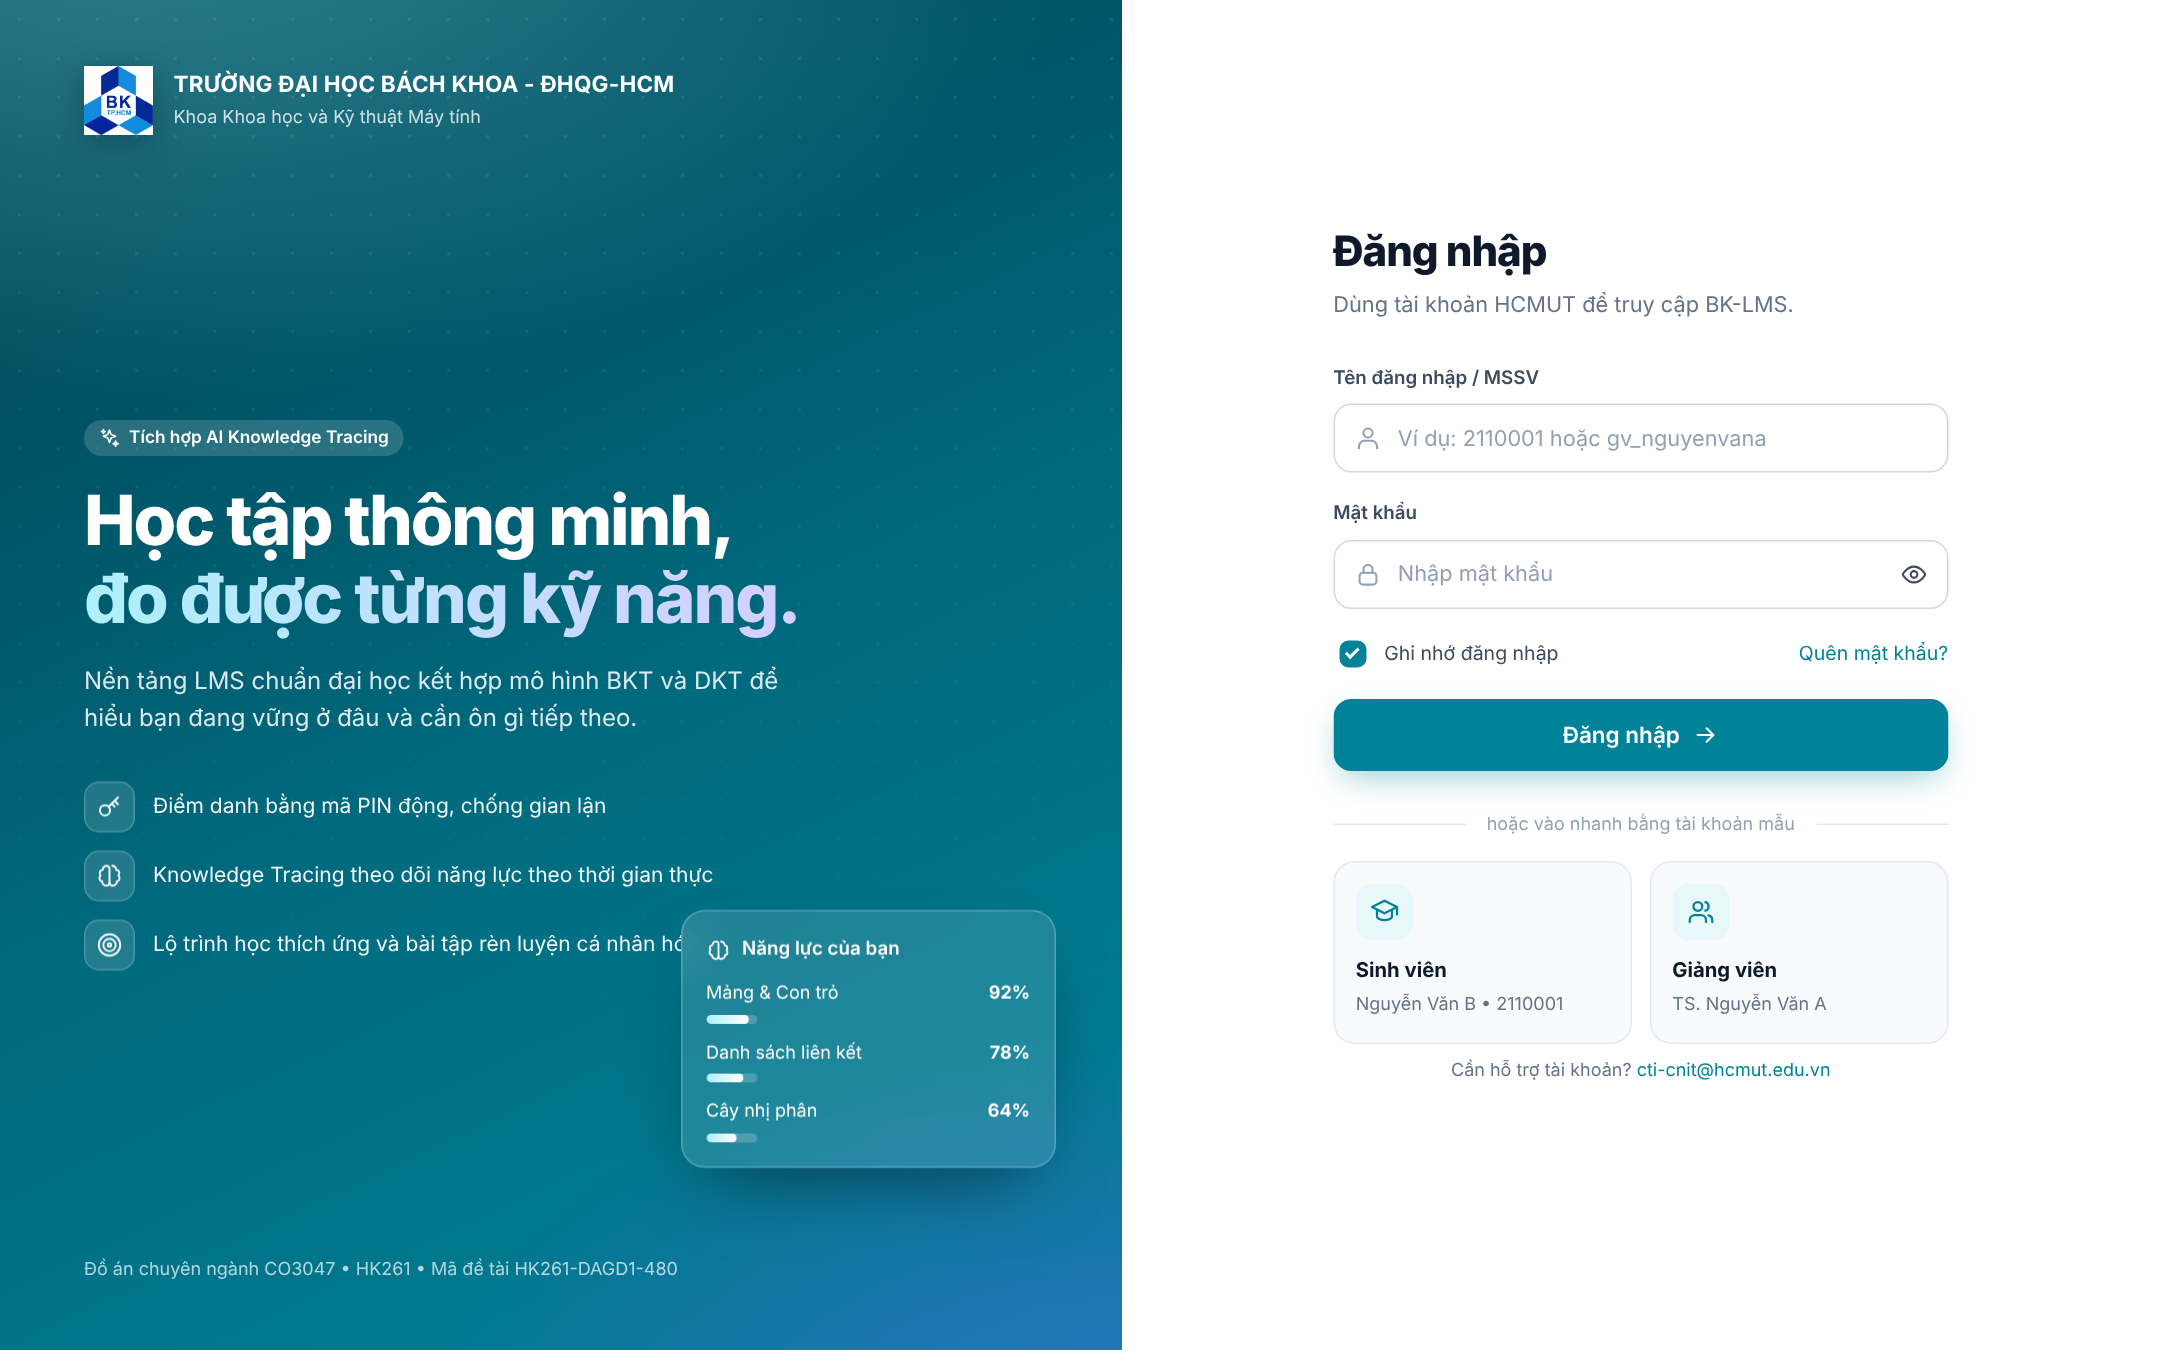
\includegraphics[width=0.6\linewidth]{images/login.png}
\caption{Login page in the style of HCMUT CAS, with separate lecturer and student entries}
\label{fig:login}
\end{figure}

\begin{figure}[H]
\centering
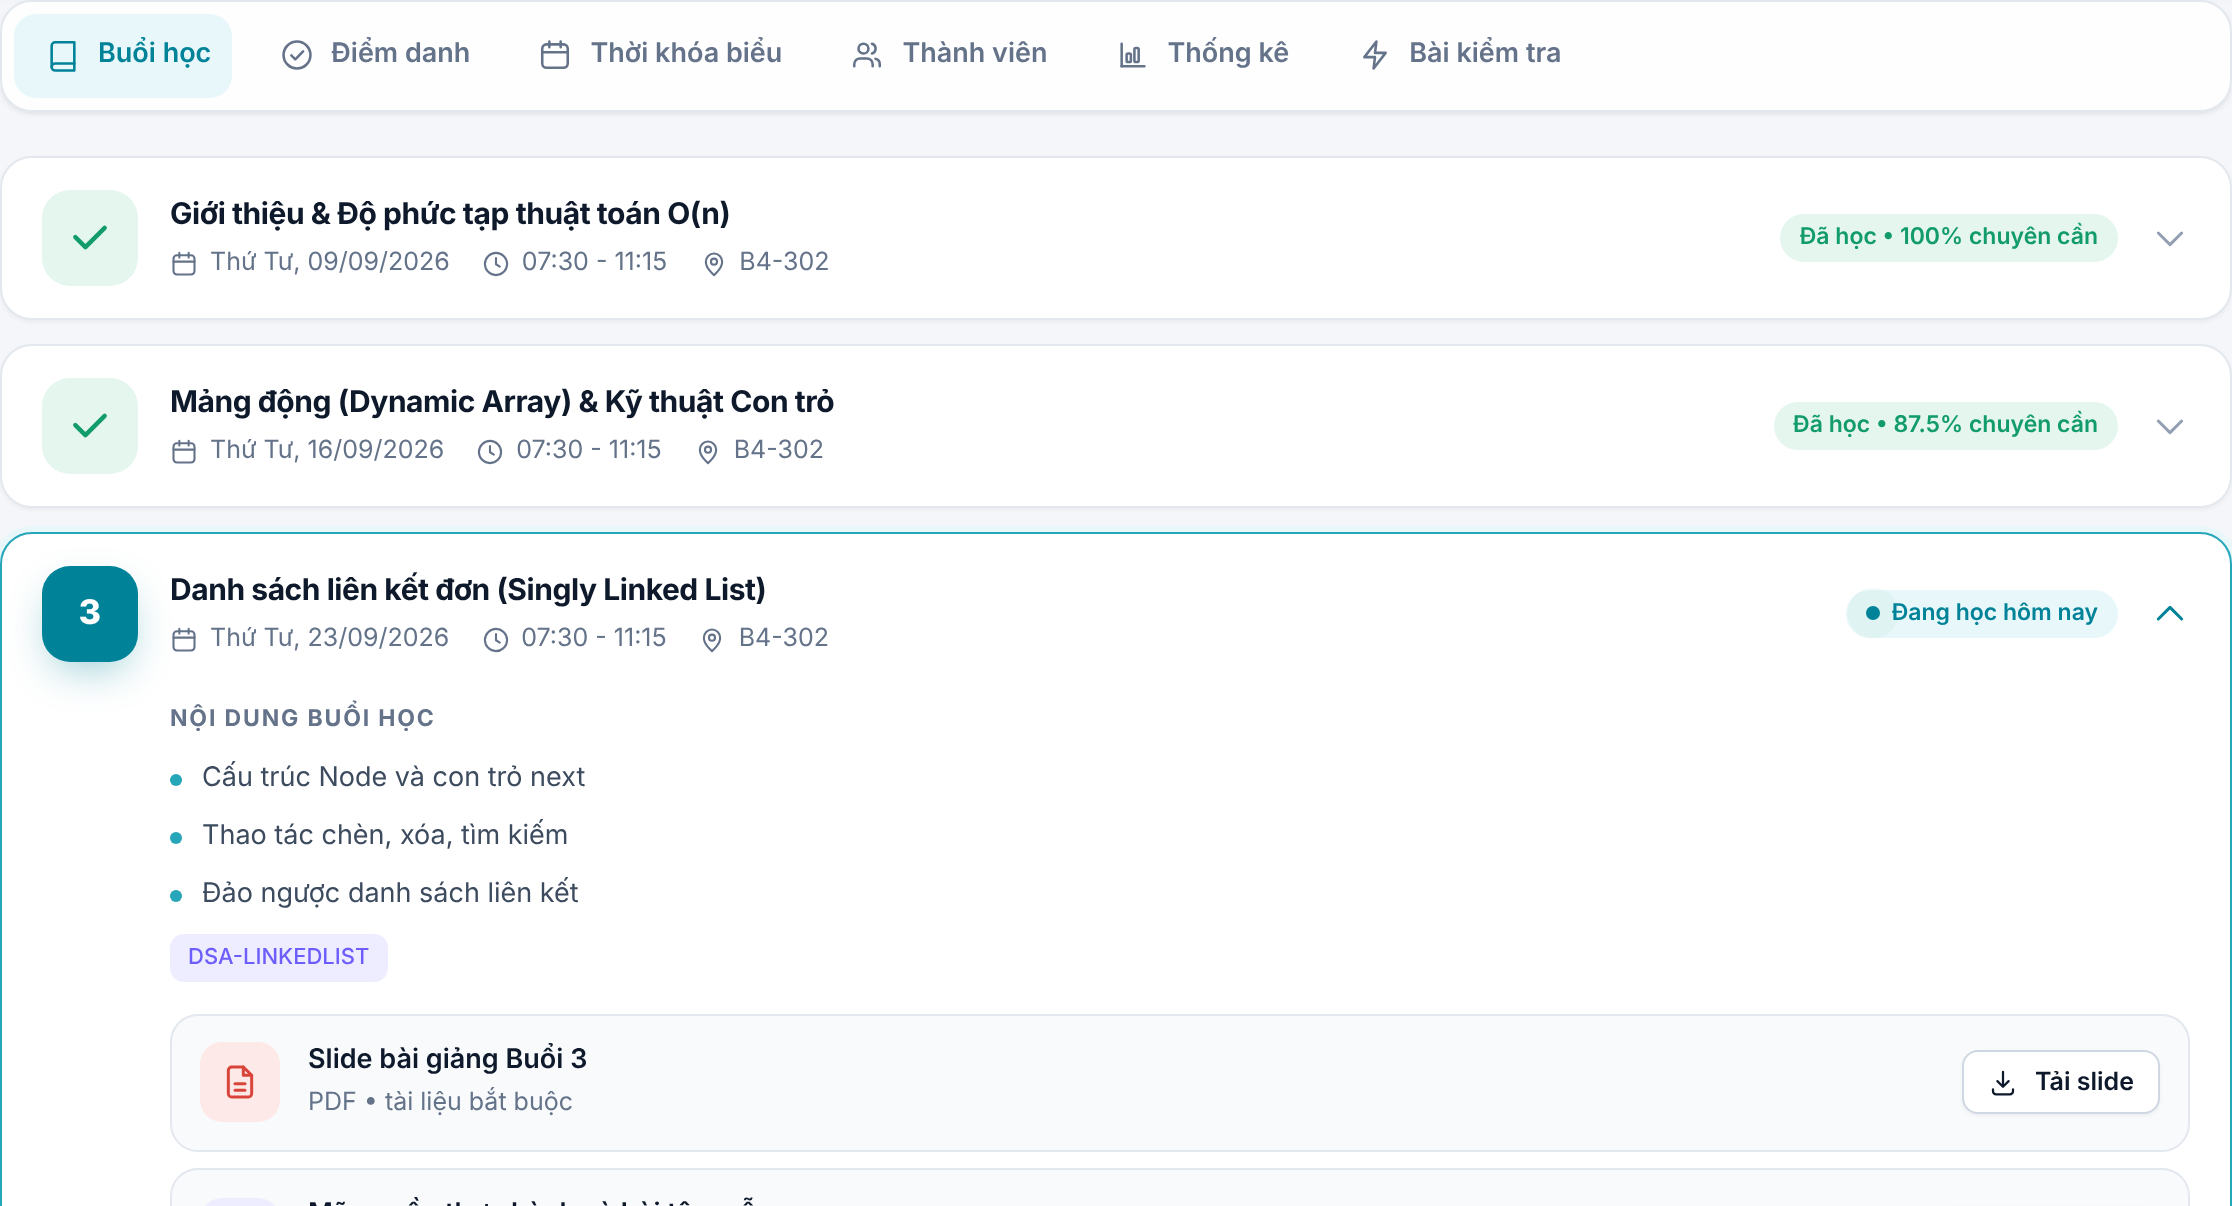
\includegraphics[width=0.82\linewidth]{images/c_sessions.png}
\caption{Course page: the fifteen sessions of CO2003 with their materials}
\label{fig:sessions}
\end{figure}

\begin{figure}[H]
\centering
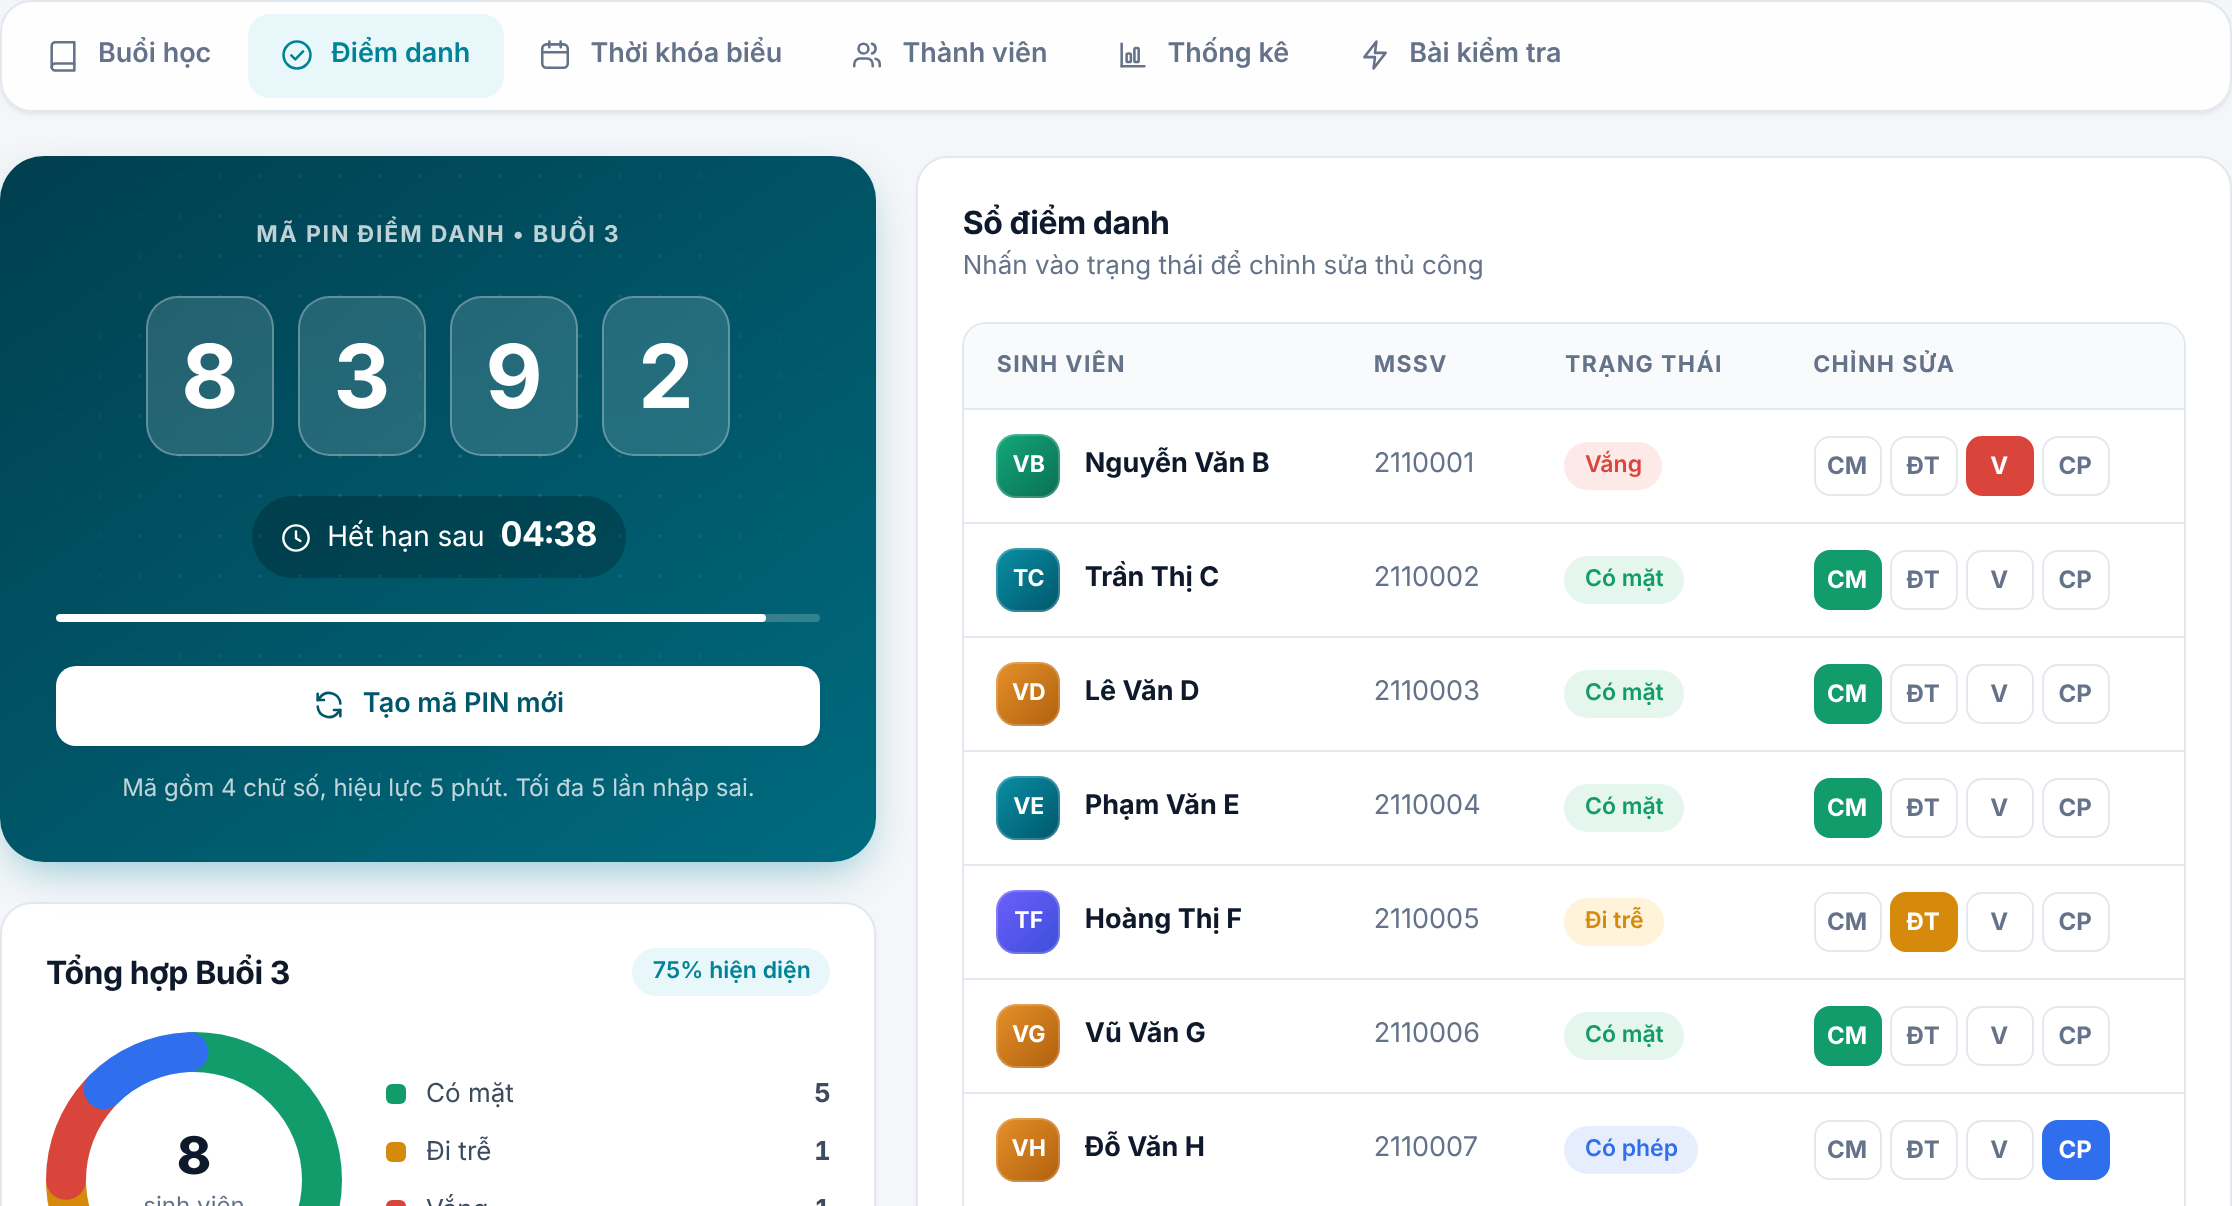
\includegraphics[width=0.82\linewidth]{images/c_attendance.png}
\caption{Attendance tab: the PIN window opened by the lecturer, with countdown and class list}
\label{fig:attendance}
\end{figure}

\begin{figure}[H]
\centering
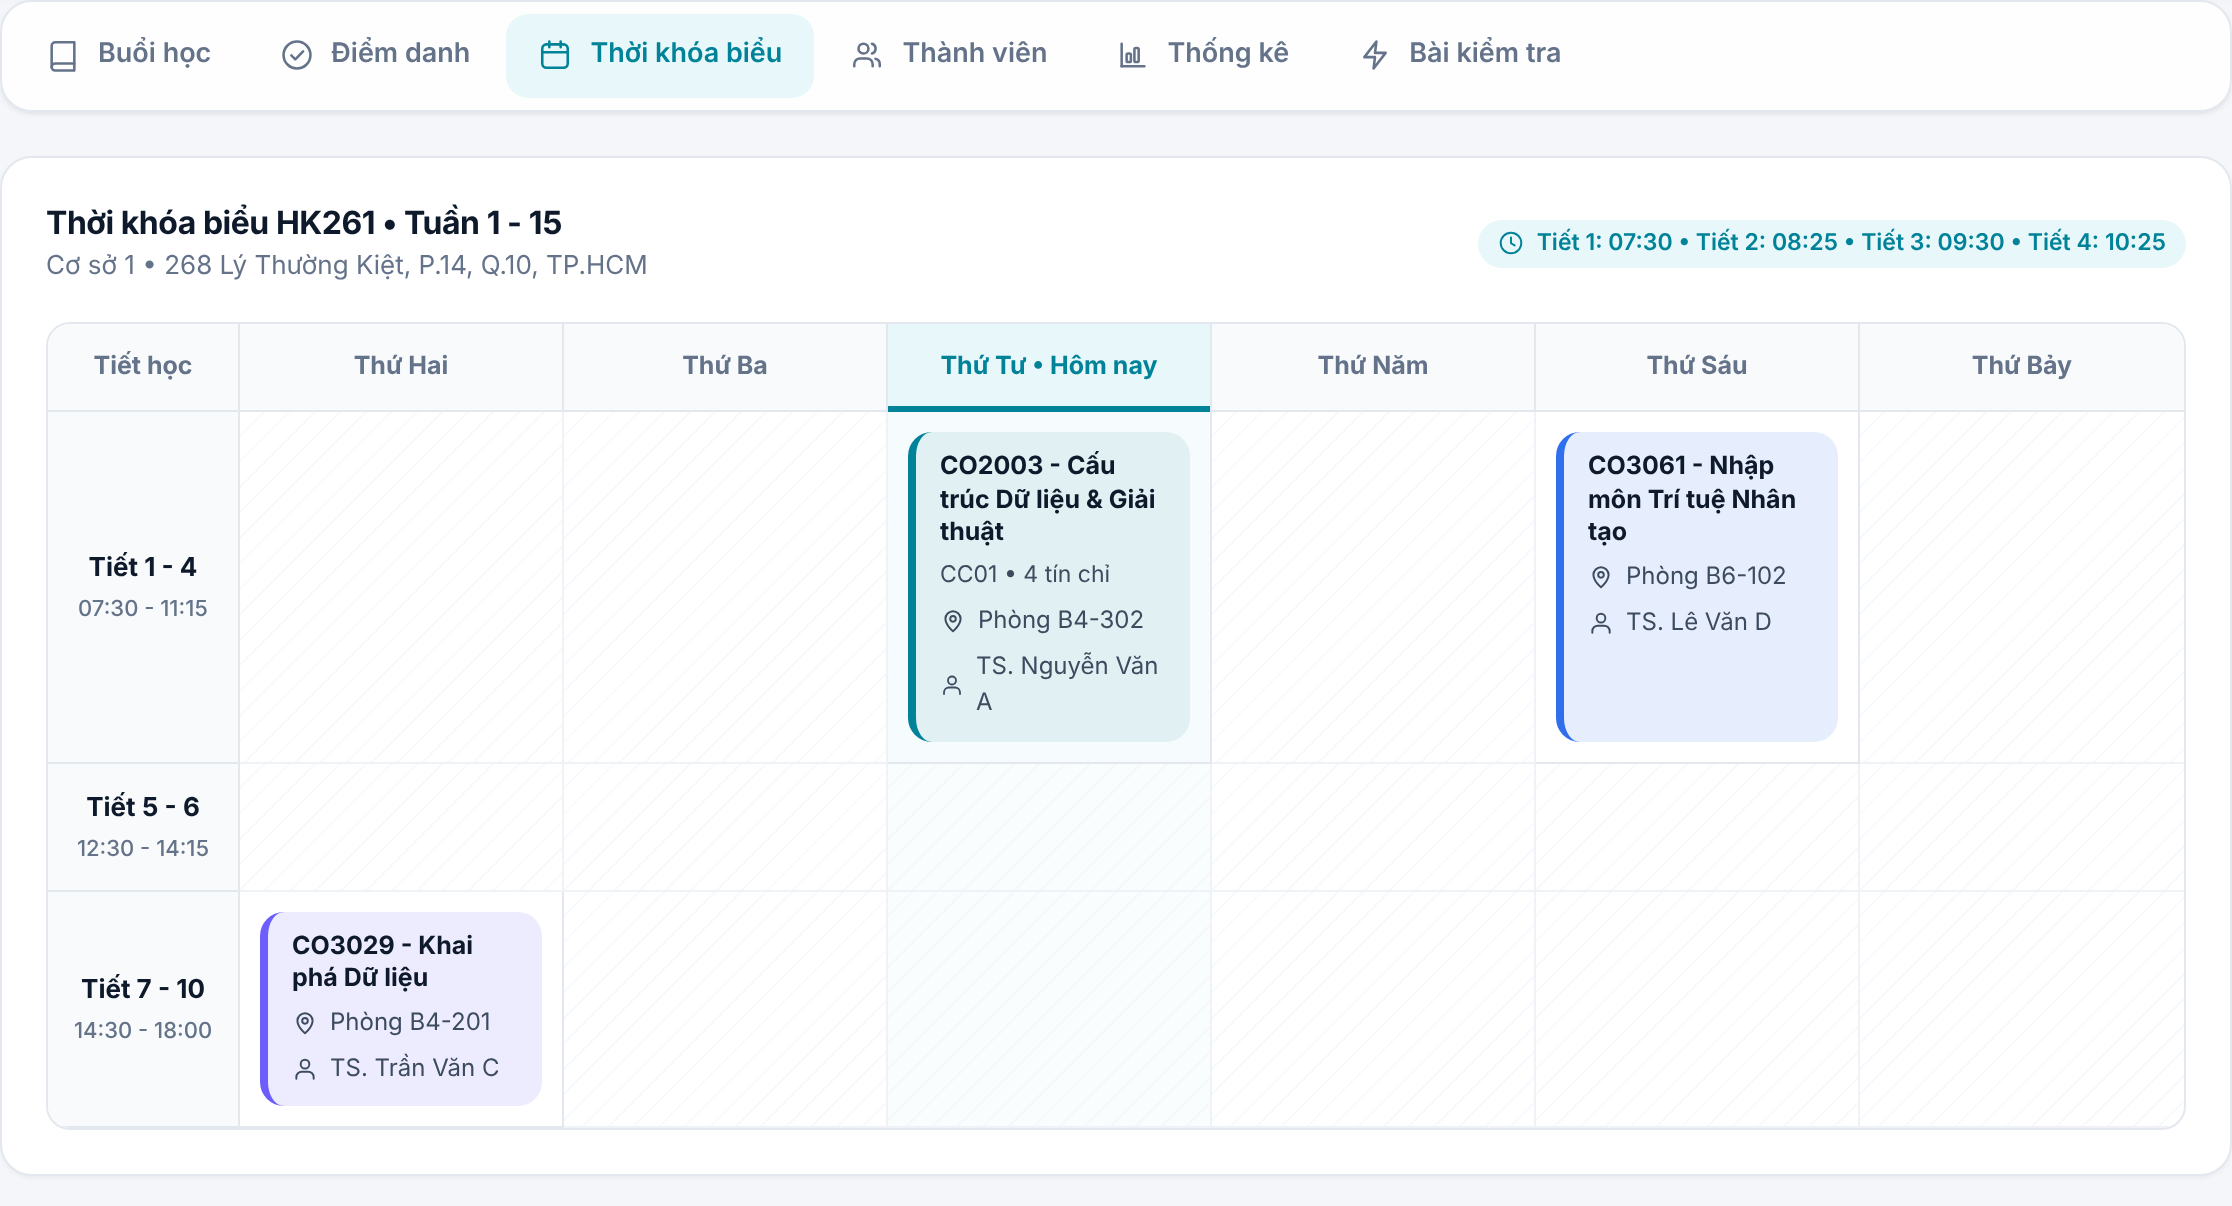
\includegraphics[width=0.82\linewidth]{images/c_timetable.png}
\caption{Weekly timetable with the current session highlighted}
\label{fig:timetable}
\end{figure}

\begin{figure}[H]
\centering
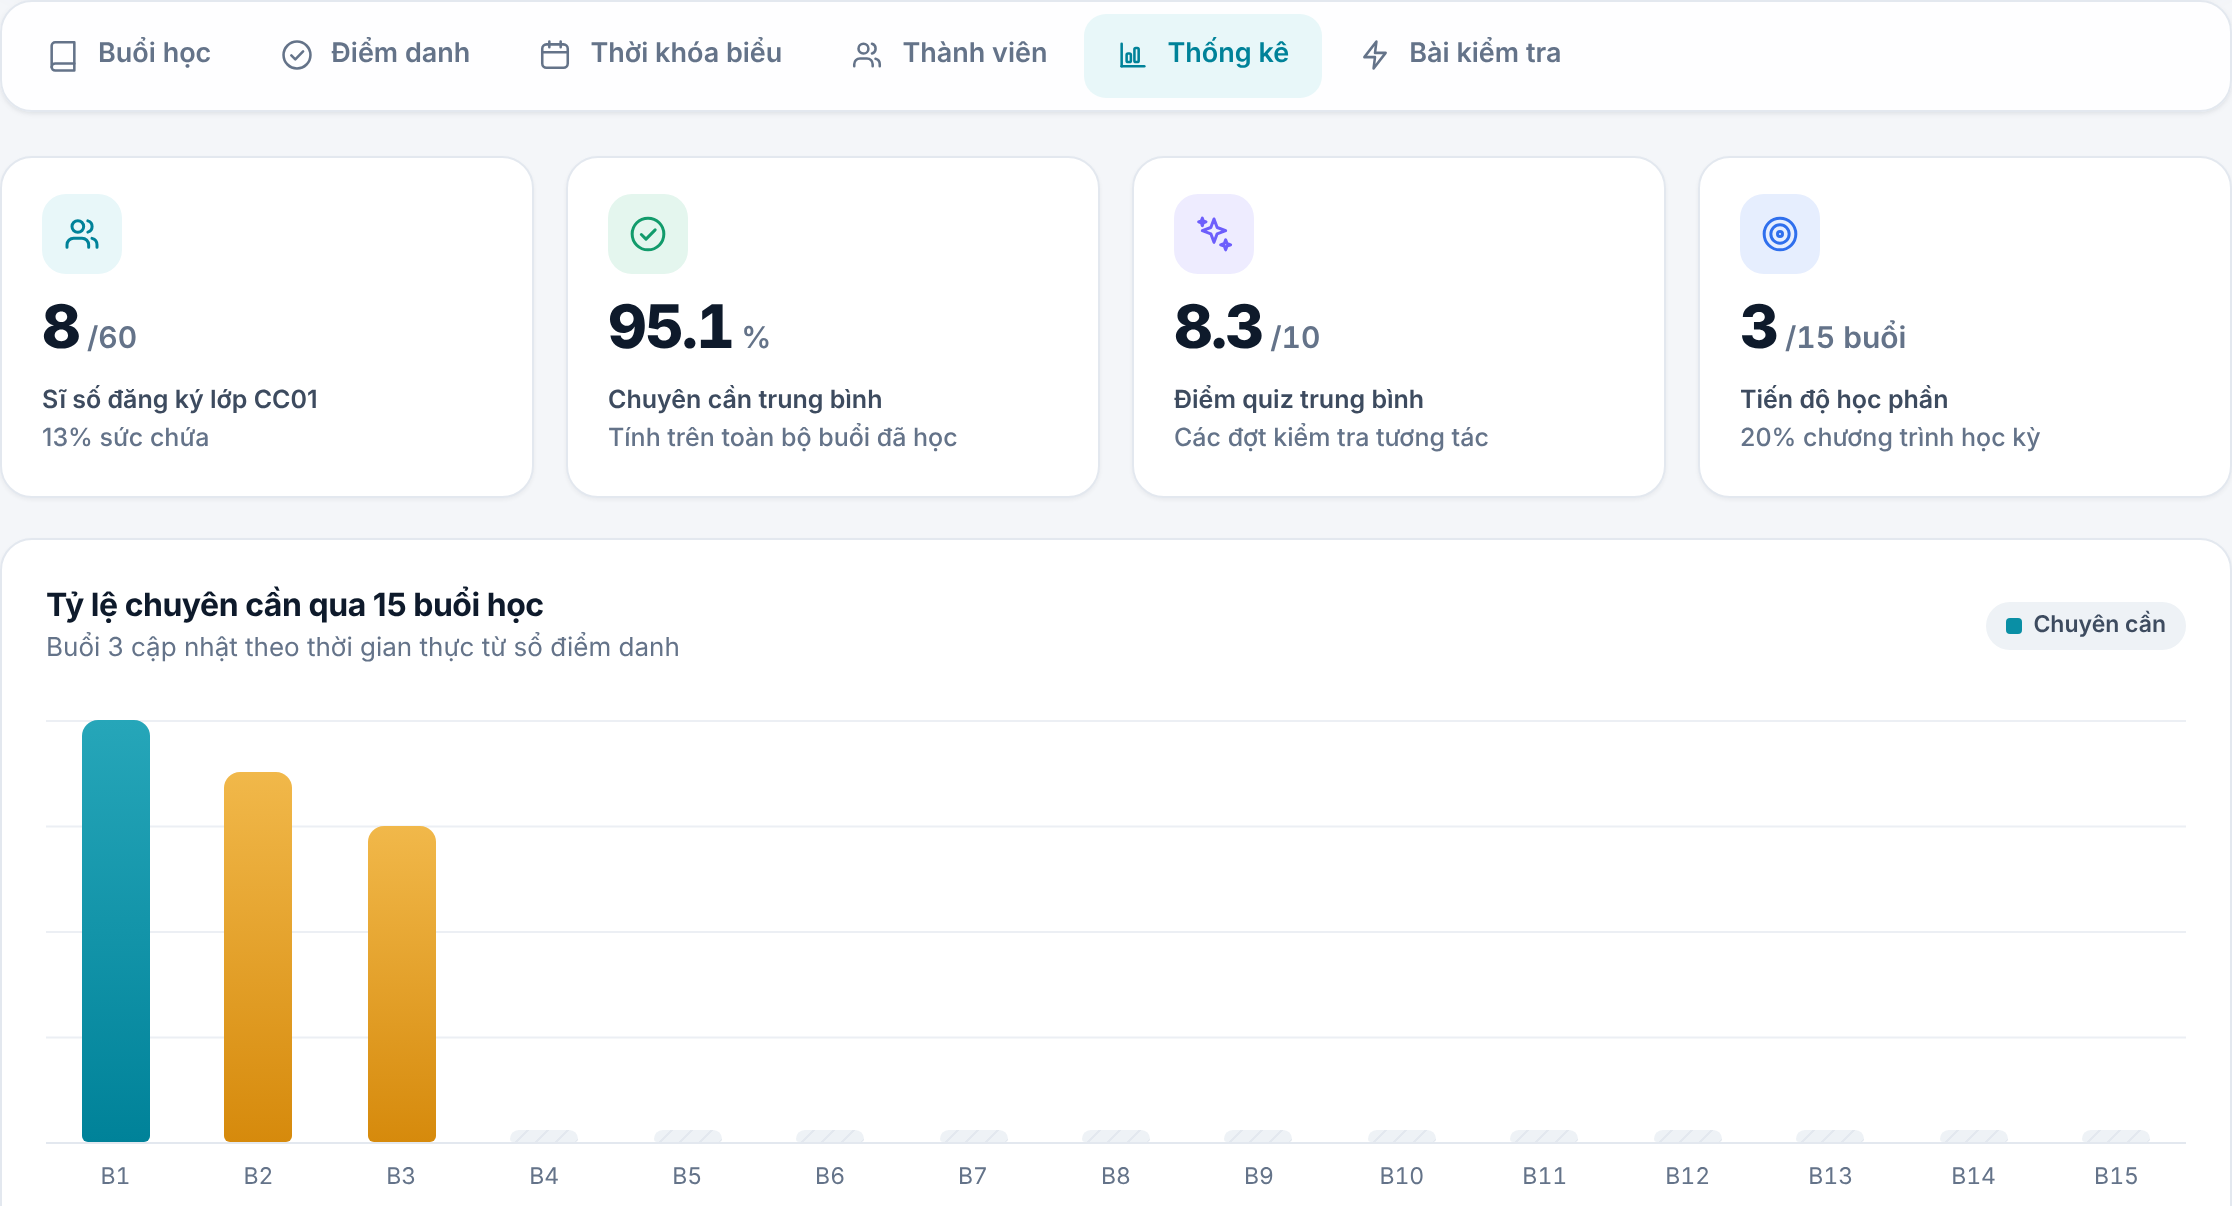
\includegraphics[width=0.82\linewidth]{images/c_stats.png}
\caption{Statistics tab: enrollment against capacity, participation per session and rate per student}
\label{fig:stats}
\end{figure}

\subsubsection{Authentication in the Prototype}

The login page separates the two roles from the first screen instead of offering a role switch on the navigation bar, which a real system would not have. Sample accounts allow the demonstration to start with one click. At the time of writing, the prototype uses data stored in the front end for its demonstration; connecting each page to the REST API is the first task of the next semester (Section~\ref{ch:plan}). We state this clearly so that the reader does not confuse the demonstration data with data coming from the database.

\subsection{Pilot Dataset: CO2003}
\label{sec:dataset}

To test the design with realistic content, the team prepared the dataset of a pilot course. The course is \emph{Data Structures and Algorithms} (CO2003, 4 credits), class CC01 of semester HK261. The dataset is stored as Markdown and JSON in the repository and can be loaded into the tables \code{course_sessions}, \code{skills}, \code{quizzes} and \code{questions}.

\subsubsection{Fifteen-Session Outline}

Table~\ref{tab:sessions} shows the outline. Each session has a title, one main skill, and a learning objective. The date of each session is computed from the start date of the semester when the data are loaded.

\begin{table}[H]
\centering
\caption{Fifteen-session outline of CO2003}
\label{tab:sessions}
\begin{tblr}{colspec={Q[c,0.9cm]Q[l,4.2cm]Q[l,3.3cm]X[l]}, row{1}={font=\bfseries}, hline{1,Z}={0.8pt}, hline{2}={0.4pt}, rowsep=2pt, rows={font=\small}}
No. & Title & Skill & Objective\\
1 & Course introduction and C++ review & \code{DSA-ARRAY} & Course goals; basic C++ and pointers\\
2 & Arrays, pointers, dynamic allocation & \code{DSA-ARRAY} & Allocate and free dynamic memory\\
3 & Algorithm complexity analysis & \code{DSA-COMPLEXITY} & Compute Big-O of simple code\\
4 & Singly linked lists & \code{DSA-LINKEDLIST} & Insert, delete, search\\
5 & Doubly and circular linked lists & \code{DSA-LINKEDLIST} & Distinguish and implement variants\\
6 & Stack & \code{DSA-STACK} & LIFO; balanced parentheses; postfix\\
7 & Queue & \code{DSA-QUEUE} & FIFO; circular queue\\
8 & Recursion & \code{DSA-RECURSION} & Base case and recursive step; cost\\
9 & Sorting & \code{DSA-SORT} & Selection, insertion, merge, quick\\
10 & Trees and binary trees & \code{DSA-TREE} & Terminology; traversals\\
11 & Binary search trees & \code{DSA-TREE} & Insert, delete, search; degenerate case\\
12 & AVL trees & \code{DSA-TREE} & Balance condition; rotations\\
13 & Heaps and priority queues & \code{DSA-HEAP} & Array heap; heap sort\\
14 & Graphs & \code{DSA-GRAPH} & Representations; BFS and DFS\\
15 & Hash tables and review & \code{DSA-HASH} & Hash functions; collisions; course review\\
\end{tblr}
\end{table}

\subsubsection{Skills and Question Bank}

The bank has 40 multiple-choice questions with four options, one correct option, a difficulty level (easy, medium, hard), a session number and a one-sentence explanation. Each question is labeled with exactly one of eleven skills. The correct answers are shuffled over the four positions to avoid a bias toward one letter. Table~\ref{tab:skills} shows the distribution.

\begin{table}[H]
\centering
\caption{Skills (knowledge components) and number of questions}
\label{tab:skills}
\begin{tblr}{colspec={Q[l,4cm]X[l]Q[r,2.2cm]}, row{1}={font=\bfseries}, hline{1,Z}={0.8pt}, hline{2}={0.4pt}, rowsep=2pt}
Skill code & Content & Questions\\
\code{DSA-ARRAY} & Arrays and pointers & 5\\
\code{DSA-COMPLEXITY} & Algorithm complexity & 1\\
\code{DSA-LINKEDLIST} & Linked lists & 6\\
\code{DSA-STACK} & Stack & 4\\
\code{DSA-QUEUE} & Queue & 3\\
\code{DSA-RECURSION} & Recursion & 1\\
\code{DSA-SORT} & Sorting & 2\\
\code{DSA-TREE} & Binary trees, BST, AVL & 8\\
\code{DSA-HEAP} & Heap & 2\\
\code{DSA-GRAPH} & Graphs & 5\\
\code{DSA-HASH} & Hash tables & 3\\
\textbf{Total} & & \textbf{40}\\
\end{tblr}
\end{table}

\paragraph{Example.} Question DSA-Q09 (session 4, skill \code{DSA-LINKEDLIST}, medium): ``To delete the node right after node $p$ (where $p\rightarrow next$ is not NULL), the correct approach is?'' The correct option is: save $q = p\rightarrow next$, set $p\rightarrow next = q\rightarrow next$, then free $q$. The explanation states that the node to delete must be saved before relinking, otherwise the reference is lost.

\paragraph{Remarks on the dataset.} The distribution is not uniform: complexity and recursion have one question each, which is too few for any statistical use. Expanding the bank to at least 3--5 questions per skill is part of the plan for HK262. The sample schedule in the dataset (Tuesday, periods 2--4, room H6-302) is a sample value and differs from the demonstration data of the prototype; both are replaced by the real timetable when the class is registered.

\subsection{Traceability: From Requirements to Code}

Table~\ref{tab:trace} shows, for every functional requirement, where it is implemented and its status at the date of this report. ``API'' means the endpoint exists in the back end; ``UI'' means a screen exists in the prototype.

\begin{table}[H]
\centering
\caption{Requirements traceability and implementation status (November 2026)}
\label{tab:trace}
\begin{tblr}{colspec={Q[l,1.2cm]X[l]Q[l,2.0cm]Q[l,2.0cm]}, row{1}={font=\bfseries}, hline{1,Z}={0.8pt}, hline{2}={0.4pt}, rowsep=2pt, rows={font=\small}}
ID & Where implemented & API & UI\\
FR1 & \code{/api/auth/*}, login page & Yes & Yes\\
FR2 & \code{/api/schedule}, course cards & Yes & Yes\\
FR3 & \code{/api/classes/:id/enroll}, trigger & Yes & Partial\\
FR4 & \code{/sessions}, \code{/sessions/bulk} & Create only & Yes\\
FR5 & \code{CHECK}/\code{UNIQUE} (number, time range); room-conflict check is not implemented yet & Partial & Partial\\
FR6 & \code{/api/schedule}, timetable tab & Yes & Yes\\
FR7 & \code{session_materials}, sessions tab & Read & Yes\\
FR8 & \code{/attendance/open} & Yes & Yes\\
FR9 & \code{/attendance/check-in} & Yes & Yes\\
FR10 & Check-in transaction & Yes & Yes\\
FR11 & \code{/attendance/close}; manual marking & Close only & Yes\\
FR12 & \code{/attendance/summary} & Yes & Yes\\
FR13 & \code{/quizzes/:id/submit} & Yes & Yes\\
FR14 & Question creation & No & No\\
FR15 & Theme variables & --- & Yes\\
\end{tblr}
\end{table}

\noindent\textit{Note.} ``UI = Yes'' means that a screen exists in the prototype. The screens currently use demonstration data kept in the front end and are not yet connected to the REST API; the connection is the first task of Section~\ref{ch:plan}.

\section{Testing, Current Status and Discussion}
\label{ch:eval}

This section reports what has been verified so far, what is still missing, and how the result compares with the requirements. We keep the three categories separate on purpose: a test that has been \emph{run}, a test that is \emph{specified but not run}, and a feature that is \emph{not implemented}.

\subsection{Test Strategy}

Testing follows the usual levels of software verification~\cite{sommerville2016software}:

\begin{itemize}
    \item \textbf{Database level.} Apply \code{schema.sql} to an empty database; verify each constraint with a statement that must fail.
    \item \textbf{API level.} Call each endpoint with valid and invalid input and with each role; verify status codes and bodies.
    \item \textbf{Concurrency level.} Fire parallel enrollment requests at a class that has one free seat, and parallel wrong-PIN requests from one student.
    \item \textbf{Interface level.} Walk through each use case in the browser in both themes and on three viewport widths.
    \item \textbf{Usability level.} Task-based test with students and a SUS questionnaire~\cite{brooke1996sus, bangor2008empirical}.
\end{itemize}

\subsection{Test Cases}

Table~\ref{tab:tests} lists the main test cases. The column ``Status'' reflects the situation at the date of this report.

\begin{table}[H]
\centering
\caption{Main test cases and status}
\label{tab:tests}
\begin{tblr}{colspec={Q[l,1.1cm]Q[l,3.6cm]X[l]Q[l,2.1cm]}, row{1}={font=\bfseries}, hline{1,Z}={0.8pt}, hline{2}={0.4pt}, rowsep=2pt, rows={font=\footnotesize}}
ID & Test & Expected result & Status\\
T1 & Apply the schema twice & Second run changes nothing and raises no error & Specified\\
T2 & Insert session number 16 & Rejected by \code{CHECK} & Specified\\
T3 & Insert a session with end before start & Rejected by \code{CHECK} & Specified\\
T4 & Set a PIN of 3 digits or without expiry & Rejected by \code{CHECK} & Specified\\
T5 & Insert two attendance records for the same student and session & Second rejected by \code{UNIQUE} & Specified\\
T6 & 61 students enroll in a class of capacity 60 (in parallel) & Exactly 60 succeed; the others fail with error 23514 & Specified\\
T7 & Student calls \code{attendance/open} & HTTP 403 & Specified\\
T8 & Check in with a correct PIN while open & HTTP 201; record status \emph{present} or \emph{late} & Specified\\
T9 & Check in after expiry & HTTP 410; PIN cleared & Specified\\
T10 & Six wrong PINs in 15 minutes & Five get 401, the sixth gets 429 & Specified\\
T11 & Check in twice with the correct PIN & Second gets 409 & Specified\\
T12 & Student fetches quiz questions & No \code{correct_answer} field in the response & Specified\\
T13 & Login with the sample lecturer and student accounts in the prototype & Role-specific home page is shown & Checked manually\\
T14 & Switch between light and dark themes and reload & Theme is kept & Checked manually\\
T15 & Open every course tab in the prototype & No error; screens render & Checked manually\\
T16 & Open the quiz tab and take a quiz of one session & Questions appear; score shown at the end & Checked manually\\
\end{tblr}
\end{table}

No automated test suite exists yet. Building one is a task of the first weeks of HK262 (Section~\ref{ch:plan}). We deliberately do not report performance figures: the target of NFR6 has not been measured.

\subsection{Evaluation Against Requirements}

Table~\ref{tab:coverage} summarizes the coverage of the use cases.

\begin{table}[H]
\centering
\caption{Coverage of use cases at the date of this report}
\label{tab:coverage}
\begin{tblr}{colspec={Q[l,1.2cm]X[l]X[l]}, row{1}={font=\bfseries}, hline{1,Z}={0.8pt}, hline{2}={0.4pt}, rowsep=3pt}
UC & Done & Missing\\
UC1 & Login and registration API; login page; course cards & Password reset; progress tracking of material views\\
UC2 & Quiz screens; submission API storing one record per answer & Offline retry; resume; timer\\
UC3 & Schema supports questions with a skill & Authoring screen and API\\
UC5 & Bulk and single creation; schedule API; timetable and sessions screens & Edit and delete; room-conflict check\\
UC6 & Open, close, check-in, rate limit, expiry sweep, record & Manual marking; regenerate PIN\\
UC7 & Summary API; statistics screen & Filters; export; threshold highlighting\\
\end{tblr}
\end{table}

\subsection{Limitations}

\begin{enumerate}
    \item The front end is not yet connected to the API; screens use demonstration data.
    \item The CAS login page is a reproduction and does not authenticate with the real HCMUT service.
    \item The PIN is stored in clear text in \code{attendance_code} while the window is open (it is cleared at close). This is acceptable for a value that lives minutes and is shown to the lecturer, but it means that anybody with read access to the database can read an active PIN. Hashing would not help because the lecturer must see the PIN.
    \item A four-digit PIN does not stop a present student from sharing it with an absent one (Section~\ref{sec:pin-security}).
    \item The question bank is in English while the interface is in Vietnamese; a bilingual bank is planned.
    \item The distribution of questions per skill is uneven (Table~\ref{tab:skills}).
    \item The room and slot of the sample timetable differ between the dataset and the demonstration data.
    \item There is no automated test suite and no performance measurement.
\end{enumerate}

\section{Conclusion and Plan for the Graduation Project (HK262)}
\label{ch:plan}

\subsection{Conclusion}

This report presented the first phase of the project ``Design of an E-Learning System with AI Integration'': a university-grade e-learning platform in the style of BKeL. We analyzed the needs of lecturers and students, specified seven use cases, and designed a three-tier architecture and a fourteen-table relational schema in third normal form. The most important design contributions are the fifteen-session model of a class, the capacity trigger with row locking, the composite foreign key that keeps quiz telemetry consistent with the skill of its question, and a PIN attendance protocol with expiry, rate limiting, constant-time comparison and one record per student and session.

The implementation consists of a typed Express API with authentication, role checks and the attendance transaction, and a Next.js prototype that reproduces the BKeL visual identity with a light and a dark theme. A pilot dataset for CO2003 provides fifteen sessions and forty skill-labeled questions. The report also states the current gaps: the front end is not connected to the API, tests are not automated, and several secondary flows (manual attendance, question authoring, session editing) are missing.

\subsection{Direction Given by the Supervisor}

After the third meeting, the supervisor asked the team to finish the e-learning system properly before extending it. The plan below follows this direction: the first eight weeks bring the system to a complete, tested state; only then are the intelligent features of the full project added, and they remain optional for the evaluation of the system itself.

\subsection{Plan for Weeks 1--15 of the Graduation Project (HK262)}

Table~\ref{tab:plan} lists the week-by-week plan. The plan is organized in five phases with a deliverable at the end of each phase. Figure~\ref{fig:gantt} gives an overview.

\begin{longtblr}[caption={Week-by-week plan for HK262}, label={tab:plan}]{colspec={Q[l,1.3cm]X[l]X[l]}, row{1}={font=\bfseries}, hline{1,Z}={0.8pt}, hline{2}={0.4pt}, rowsep=2pt, rows={font=\small}}
Week & Tasks & Deliverable\\
1 & Review feedback on this report; freeze scope of phase~1; write an OpenAPI description of all endpoints; set up Docker Compose (PostgreSQL, API, front end) & API specification; one-command local environment\\
2 & Connect login, registration and the course list to the API; replace demonstration data by API data; error and loading states & Working login and course list on real data\\
3 & Connect sessions, timetable and enrollment; bulk session creation from the lecturer screen; room-conflict check & Schedule module end to end\\
4 & Connect PIN attendance (open, close, check-in) and statistics; add the live list refresh; manual marking and PIN regeneration & Attendance module end to end; feature freeze of phase~1\\
5 & Question authoring (UC3): create, edit, delete questions with skill labels; import of the CO2003 bank into the database; bilingual questions & Question bank module\\
6 & Automated tests: SQL constraint tests, API tests for every endpoint and role, concurrency tests (enrollment, PIN attempts) & Test suite in continuous integration\\
7 & Security review against the OWASP verification checklist; rate limit on login; password reset flow; audit of error messages & Security review report\\
8 & Performance measurement of the main endpoints with 60 and 300 simulated students; indexes tuned from query plans & Measured results for NFR6\\
9 & Design of the learning-support extension: student competency view built from quiz history (UC4); definition of skill model and data export from \code{quiz_interactions} & Design document of the extension\\
10 & Implementation of a first baseline for per-skill mastery estimation from quiz history, with a fallback to empirical accuracy & Baseline estimator service\\
11 & Integration of the estimator into the student view; recommendations of sessions to review; expansion of the question bank to 3--5 questions per skill & Competency view in the course page\\
12 & Usability study with 8--10 students and 2 lecturers: tasks, observation, SUS questionnaire~\cite{brooke1996sus} & Study protocol; raw data\\
13 & Analysis of the study; fixes of the most serious problems; accessibility check with WCAG 2.1 criteria~\cite{wcag21} & Study report; fixed issues\\
14 & Deployment on a test server (HTTPS, environment variables, backups); user guide and administrator guide & Deployed system; manuals\\
15 & Final report, slides and demonstration; rehearsal of the defense & Final report; defense package\\
\end{longtblr}

\begin{figure}[H]
\centering
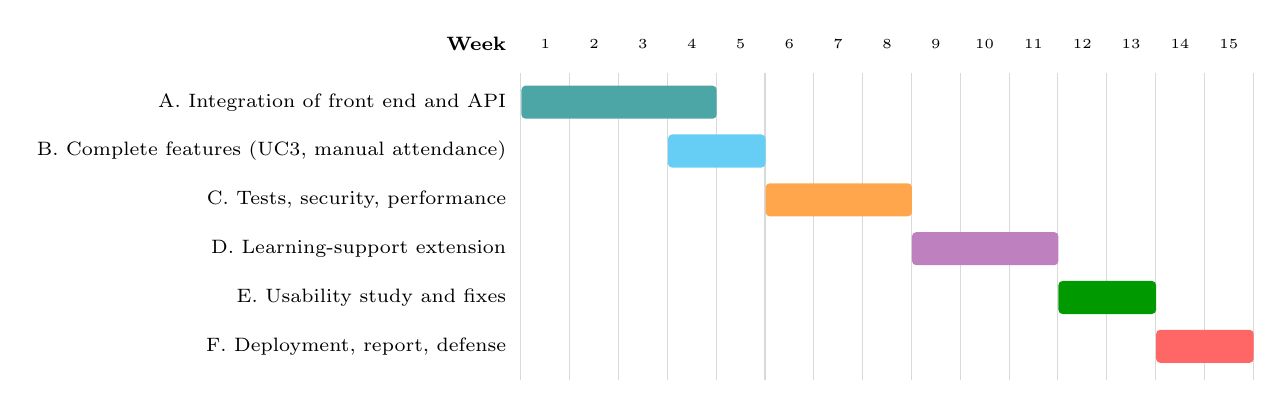
\begin{tikzpicture}[x=0.62cm, y=0.62cm,
    bar/.style={rectangle, rounded corners=1.5pt, minimum height=0.42cm, inner sep=0pt},
    >=stealth]
\foreach \w in {1,...,15} {
    \node[font=\tiny] at (\w-0.5+4.2,0.6) {\w};
    \draw[gray!30] (\w+4.2,0) -- (\w+4.2,-6.3);
}
\draw[gray!30] (4.2,0) -- (4.2,-6.3);
\node[font=\scriptsize\bfseries, anchor=east] at (4.1,0.6) {Week};
\def\rowitem#1#2#3#4#5{%
  \node[font=\scriptsize, anchor=east] at (4.1,-#1) {#2};
  \node[bar, fill=#5, anchor=west, minimum width={(#4-#3+1)*0.62cm}] at (#3+3.2,-#1) {};}
\rowitem{0.6}{A. Integration of front end and API}{1}{4}{teal!70}
\rowitem{1.6}{B. Complete features (UC3, manual attendance)}{4}{5}{cyan!60}
\rowitem{2.6}{C. Tests, security, performance}{6}{8}{orange!70}
\rowitem{3.6}{D. Learning-support extension}{9}{11}{violet!50}
\rowitem{4.6}{E. Usability study and fixes}{12}{13}{green!60!black}
\rowitem{5.6}{F. Deployment, report, defense}{14}{15}{red!60}
\end{tikzpicture}
\caption{Overview of the plan for HK262 (weeks 1--15)}
\label{fig:gantt}
\end{figure}

\subsection{Planned Meetings and Report Milestones}

Meetings with the supervisor are held every two weeks, with an optional Friday afternoon session on request. The milestones for the report of the current semester are 15 November 2026 (at least 30 pages), 30 November 2026 (at least 50 pages) and 15 December 2026 (at least 70 pages). The final defense is on 31 December 2026.

\subsection{Intelligent Learning Support: Background for Weeks 9--11}

The extension of weeks 9--11 builds on the field of knowledge tracing, which models the knowledge state of a learner from the sequence of answers. The classical model, Bayesian Knowledge Tracing, estimates for each skill the probability that the learner has mastered it~\cite{corbett1995knowledge}; neural variants, introduced with Deep Knowledge Tracing, predict the probability of a correct answer from the whole sequence~\cite{piech2015deep}. The data model of the first phase already stores what these methods need: one row per answer with the user, the skill, the correctness and the time. The decision about which model to use will be taken in week~9 after reviewing the amount of data that can be collected; with a small number of students, a simple and interpretable baseline is more appropriate than a neural model. This part is explicitly separated from the evaluation of the e-learning system itself.


\clearpage
\phantomsection
\addcontentsline{toc}{section}{References}
\renewcommand{\refname}{References}
\begin{thebibliography}{99}
\setlength{\itemsep}{0.4em}
\bibitem{ellis2009field} R. K. Ellis, \textit{Field Guide to Learning Management Systems}, ASTD Learning Circuits, 2009.
\bibitem{kasim2016choosing} N. N. M. Kasim and F. Khalid, ``Choosing the Right Learning Management System ({LMS}) for the Higher Education Institution Context: A Systematic Review,'' \textit{International Journal of Emerging Technologies in Learning}, vol.~11, no.~6, pp.~55--61, 2016.
\bibitem{dougiamas2003moodle} M. Dougiamas and P. C. Taylor, ``Moodle: Using Learning Communities to Create an Open Source Course Management System,'' in \textit{Proceedings of EDMEDIA 2003}, 2003.
\bibitem{crede2010class} M. Cred{\'e}, S. G. Roch, and U. M. Kieszczynka, ``Class Attendance in College: A Meta-Analytic Review of the Relationship of Class Attendance With Grades and Student Characteristics,'' \textit{Review of Educational Research}, vol.~80, no.~2, pp.~272--295, 2010.
\bibitem{kassarnig2018academic} V. Kassarnig, E. Mones, A. Bjerre-Nielsen, P. Sapiezynski, D. Dreyer Lassen, and S. Lehmann, ``Academic Performance and Behavioral Patterns,'' \textit{EPJ Data Science}, vol.~7, no.~1, pp.~10, 2018.
\bibitem{alfraihat2020evaluating} D. Al-Fraihat, M. Joy, R. Masa'deh, and J. Sinclair, ``Evaluating {E-learning} Systems Success: An Empirical Study,'' \textit{Computers in Human Behavior}, vol.~102, pp.~67--86, 2020.
\bibitem{moodledocs} Moodle Pty Ltd, ``Moodle Documentation,'' 2024. [Online]. Available: \url{https://docs.moodle.org}
\bibitem{rfc6585} M. Nottingham and R. Fielding, ``Additional {HTTP} Status Codes,'' IETF, RFC~6585, 2012. [Online]. Available: \url{https://www.rfc-editor.org/rfc/rfc6585}
\bibitem{bass2021software} L. Bass, P. Clements, and R. Kazman, \textit{Software Architecture in Practice}, 4th ed., Addison-Wesley, 2021.
\bibitem{fowler2002patterns} M. Fowler, \textit{Patterns of Enterprise Application Architecture}, Addison-Wesley, 2002.
\bibitem{fielding2000architectural} R. T. Fielding, ``Architectural Styles and the Design of Network-based Software Architectures,'' Ph.D. dissertation, University of California, Irvine, 2000.
\bibitem{rfc8259} T. Bray, ``The {JavaScript} Object Notation ({JSON}) Data Interchange Format,'' IETF, RFC~8259, 2017. [Online]. Available: \url{https://www.rfc-editor.org/rfc/rfc8259}
\bibitem{rfc9110} R. Fielding, M. Nottingham, and J. Reschke, ``{HTTP} Semantics,'' IETF, RFC~9110, 2022. [Online]. Available: \url{https://www.rfc-editor.org/rfc/rfc9110}
\bibitem{rfc7519} M. Jones, J. Bradley, and N. Sakimura, ``{JSON} {Web} {Token} ({JWT}),'' IETF, RFC~7519, 2015. [Online]. Available: \url{https://www.rfc-editor.org/rfc/rfc7519}
\bibitem{provos1999bcrypt} N. Provos and D. Mazi{\`e}res, ``A Future-Adaptable Password Scheme,'' in \textit{Proceedings of the USENIX Annual Technical Conference}, pp.~81--91, 1999.
\bibitem{nist80063b} P. A. Grassi, M. E. Garcia, and J. L. Fenton, ``Digital Identity Guidelines: Authentication and Lifecycle Management,'' National Institute of Standards and Technology, NIST Special Publication 800-63B, 2017.
\bibitem{owaspasvs} OWASP Foundation, ``Application Security Verification Standard 4.0,'' 2019. [Online]. Available: \url{https://owasp.org/www-project-application-security-verification-standard/}
\bibitem{codd1970relational} E. F. Codd, ``A Relational Model of Data for Large Shared Data Banks,'' \textit{Communications of the ACM}, vol.~13, no.~6, pp.~377--387, 1970.
\bibitem{chen1976entity} P. P. S. Chen, ``The Entity-Relationship Model---Toward a Unified View of Data,'' \textit{ACM Transactions on Database Systems}, vol.~1, no.~1, pp.~9--36, 1976.
\bibitem{silberschatz2019database} A. Silberschatz, H. F. Korth, and S. Sudarshan, \textit{Database System Concepts}, 7th ed., McGraw-Hill, 2019.
\bibitem{elmasri2015fundamentals} R. Elmasri and S. B. Navathe, \textit{Fundamentals of Database Systems}, 7th ed., Pearson, 2015.
\bibitem{berenson1995critique} H. Berenson, P. Bernstein, J. Gray, J. Melton, E. O'Neil, and P. O'Neil, ``A Critique of {ANSI} {SQL} Isolation Levels,'' in \textit{Proceedings of the ACM SIGMOD International Conference on Management of Data}, pp.~1--10, 1995.
\bibitem{bernstein1981concurrency} P. A. Bernstein and N. Goodman, ``Concurrency Control in Distributed Database Systems,'' \textit{ACM Computing Surveys}, vol.~13, no.~2, pp.~185--221, 1981.
\bibitem{postgresdocs} PostgreSQL Global Development Group, ``{PostgreSQL} 15 Documentation,'' 2022. [Online]. Available: \url{https://www.postgresql.org/docs/15/}
\bibitem{nextjsdocs} Vercel, ``Next.js Documentation: App Router,'' 2024. [Online]. Available: \url{https://nextjs.org/docs}
\bibitem{reactdocs} Meta Open Source, ``React Documentation,'' 2024. [Online]. Available: \url{https://react.dev}
\bibitem{nodedocs} OpenJS Foundation, ``Node.js Documentation,'' 2024. [Online]. Available: \url{https://nodejs.org/docs/latest/api/}
\bibitem{expressdocs} OpenJS Foundation, ``Express: Fast, Unopinionated, Minimalist Web Framework for {Node.js},'' 2024. [Online]. Available: \url{https://expressjs.com}
\bibitem{typescriptdocs} Microsoft, ``{TypeScript} Documentation,'' 2024. [Online]. Available: \url{https://www.typescriptlang.org/docs/}
\bibitem{owasptop10} OWASP Foundation, ``{OWASP} Top 10: 2021,'' 2021. [Online]. Available: \url{https://owasp.org/Top10/}
\bibitem{chacon2014progit} S. Chacon and B. Straub, \textit{Pro Git}, 2nd ed., Apress, 2014.
\bibitem{beck2001agile} K. Beck and others, ``Manifesto for Agile Software Development,'' 2001. [Online]. Available: \url{https://agilemanifesto.org}
\bibitem{sommerville2016software} I. Sommerville, \textit{Software Engineering}, 10th ed., Pearson, 2016.
\bibitem{merkel2014docker} D. Merkel, ``Docker: Lightweight {Linux} Containers for Consistent Development and Deployment,'' \textit{Linux Journal}, vol.~2014, no.~239, 2014.
\bibitem{humble2010continuous} J. Humble and D. Farley, \textit{Continuous Delivery}, Addison-Wesley, 2010.
\bibitem{nielsen1993usability} J. Nielsen, \textit{Usability Engineering}, Academic Press, 1993.
\bibitem{wcag21} World Wide Web Consortium, ``Web Content Accessibility Guidelines ({WCAG}) 2.1,'' 2018. [Online]. Available: \url{https://www.w3.org/TR/WCAG21/}
\bibitem{brooke1996sus} J. Brooke, ``{SUS}: A ``Quick and Dirty'' Usability Scale,'' in \textit{Usability Evaluation in Industry}, Taylor \& Francis, 1996, pp.~189--194.
\bibitem{bangor2008empirical} A. Bangor, P. T. Kortum, and J. T. Miller, ``An Empirical Evaluation of the System Usability Scale,'' \textit{International Journal of Human--Computer Interaction}, vol.~24, no.~6, pp.~574--594, 2008.
\bibitem{cockburn2001writing} A. Cockburn, \textit{Writing Effective Use Cases}, Addison-Wesley, 2001.
\bibitem{jacobson1992object} I. Jacobson, M. Christerson, P. Jonsson, and G. {\"O}vergaard, \textit{Object-Oriented Software Engineering: A Use Case Driven Approach}, Addison-Wesley, 1992.
\bibitem{fowler2004uml} M. Fowler, \textit{{UML} Distilled: A Brief Guide to the Standard Object Modeling Language}, 3rd ed., Addison-Wesley, 2004.
\bibitem{corbett1995knowledge} A. T. Corbett and J. R. Anderson, ``Knowledge Tracing: Modeling the Acquisition of Procedural Knowledge,'' \textit{User Modeling and User-Adapted Interaction}, vol.~4, no.~4, pp.~253--278, 1995.
\bibitem{piech2015deep} C. Piech, J. Bassen, J. Huang, S. Ganguli, M. Sahami, L. J. Guibas, and J. Sohl-Dickstein, ``Deep Knowledge Tracing,'' in \textit{Advances in Neural Information Processing Systems 28}, pp.~505--513, 2015.
\end{thebibliography}
\clearpage



\end{document}
